\documentclass[a4paper,10pt]{article}\usepackage[]{graphicx}\usepackage[]{xcolor}
% maxwidth is the original width if it is less than linewidth
% otherwise use linewidth (to make sure the graphics do not exceed the margin)
\makeatletter
\def\maxwidth{ %
  \ifdim\Gin@nat@width>\linewidth
    \linewidth
  \else
    \Gin@nat@width
  \fi
}
\makeatother

\definecolor{fgcolor}{rgb}{0.345, 0.345, 0.345}
\newcommand{\hlnum}[1]{\textcolor[rgb]{0.686,0.059,0.569}{#1}}%
\newcommand{\hlstr}[1]{\textcolor[rgb]{0.192,0.494,0.8}{#1}}%
\newcommand{\hlcom}[1]{\textcolor[rgb]{0.678,0.584,0.686}{\textit{#1}}}%
\newcommand{\hlopt}[1]{\textcolor[rgb]{0,0,0}{#1}}%
\newcommand{\hlstd}[1]{\textcolor[rgb]{0.345,0.345,0.345}{#1}}%
\newcommand{\hlkwa}[1]{\textcolor[rgb]{0.161,0.373,0.58}{\textbf{#1}}}%
\newcommand{\hlkwb}[1]{\textcolor[rgb]{0.69,0.353,0.396}{#1}}%
\newcommand{\hlkwc}[1]{\textcolor[rgb]{0.333,0.667,0.333}{#1}}%
\newcommand{\hlkwd}[1]{\textcolor[rgb]{0.737,0.353,0.396}{\textbf{#1}}}%
\let\hlipl\hlkwb

\usepackage{framed}
\makeatletter
\newenvironment{kframe}{%
 \def\at@end@of@kframe{}%
 \ifinner\ifhmode%
  \def\at@end@of@kframe{\end{minipage}}%
  \begin{minipage}{\columnwidth}%
 \fi\fi%
 \def\FrameCommand##1{\hskip\@totalleftmargin \hskip-\fboxsep
 \colorbox{shadecolor}{##1}\hskip-\fboxsep
     % There is no \\@totalrightmargin, so:
     \hskip-\linewidth \hskip-\@totalleftmargin \hskip\columnwidth}%
 \MakeFramed {\advance\hsize-\width
   \@totalleftmargin\z@ \linewidth\hsize
   \@setminipage}}%
 {\par\unskip\endMakeFramed%
 \at@end@of@kframe}
\makeatother

\definecolor{shadecolor}{rgb}{.97, .97, .97}
\definecolor{messagecolor}{rgb}{0, 0, 0}
\definecolor{warningcolor}{rgb}{1, 0, 1}
\definecolor{errorcolor}{rgb}{1, 0, 0}
\newenvironment{knitrout}{}{} % an empty environment to be redefined in TeX

\usepackage{alltt}
\usepackage[T1]{fontenc}
%\usepackage[utf8]{inputenc}
%\usepackage[spanish]{babel}
\usepackage{hyperref}
\usepackage{amsmath}
\usepackage{amssymb}
\usepackage{amsfonts}
\usepackage{underscore}
\usepackage{bbm}

%\usepackage{graphicx}
%\usepackage{pstricks}

\setlength{\oddsidemargin}{0pt} \setlength{\evensidemargin}{0pt}
\setlength{\marginparwidth}{1in} \setlength{\marginparsep}{0pt}

\setlength{\topmargin}{0pt} \setlength{\headheight}{0pt}
\setlength{\headsep}{0pt} \setlength{\topskip}{0pt}

% \footheight 0pt
% \footskip 0pt
% A4 is 29,7301778cm x 21,0224103cm
%     =  9,7047944in x 6,2765395in
\setlength{\textheight}{24,6501778cm}
\setlength{\textwidth}{15,9424103cm}

\setlength{\parindent}{0pt}

\pagestyle{plain}

\title{Selection of L-shaped genes using a heuristic algorithm}
\author{S\'anchez-Pla, Alex$^{1,3}$, Mir\'o, Berta$^3$, Carmona, Francesc$^1$, \\ Bazzoco, Sara$^2$, Arango, Diego$^2$\\
  $^1$ Departament of Genetics Microbiology and Statistics, Universitat de Barcelona\\
  $^2$ CIBBIM-Nanomedicine. Biomedical Research in Digestive Tumors, (VHIR), Barcelona\\
  $^3$ Statistic and Bioinformatics Unit. Vall d'Hebron Research Institute.  (VHIR). Barcelona}
\date{}
\IfFileExists{upquote.sty}{\usepackage{upquote}}{}
\begin{document}
%\SweaveOpts{concordance=TRUE}



\maketitle

\thispagestyle{empty}

\tableofcontents

\section{Introduction}

This document contains examples / applications on how to select L-shaped genes from two data matrices, an expression and a methylation matrix, matched by rows (genes) and columns(samplea), using the algorithms implemented by the authors and described elsewhere.
 

The idea is to "keep-it-simple" so that it can serve as the basis for other applications such as a program that optimizes the parameters or for a graphical user interface based in Shiny.

Essentially what the program does is
\begin{itemize}
  \item Data input
  \begin{itemize} 
    \item Select (Load) expression values from a csv file
    \item Select (Load) methylation values from a csv file
    \item Data preprocessing may need to be done automatically so that its results can be used for filtering.
    \item Set parameter values
    \begin{itemize}
      \item For data use (all genes or only those that pass certain filters (corr < 0))
      \item For L-shape selection method: Here one may want to select the method and its parameters (each method has a different set of parameters)
    \end{itemize}
  \end{itemize}
  \item Data processing (For each method and set of parameters ...)
  \begin{itemize} 
    \item Run the computation and "mark" L-shape genes
    \item Draw the scatterplots of either all genes or only selected genes
  \end{itemize}
  \item Data output (For each method and set of parameters ...)
  \begin{itemize} 
    \item Save (Download) the resulting gene list(s)
    \item Save (Download) the scatterplots 
  \end{itemize}
\end{itemize}



\begin{knitrout}
\definecolor{shadecolor}{rgb}{0.969, 0.969, 0.969}\color{fgcolor}\begin{kframe}
\begin{alltt}
\hlkwa{if} \hlstd{(}\hlopt{!}\hlstd{(}\hlkwd{require}\hlstd{(VennDiagram)))} \hlkwd{install.packages}\hlstd{(}\hlstr{"VennDiagram"}\hlstd{)}
\hlkwa{if} \hlstd{(}\hlopt{!}\hlstd{(}\hlkwd{require}\hlstd{(org.Hs.eg.db)))}
  \hlstd{biocManager}\hlopt{::}\hlkwd{install}\hlstd{(}\hlstr{"org.Hs.eg.db"}\hlstd{)}
\hlkwa{if}\hlstd{(}\hlopt{!}\hlstd{(}\hlkwd{require}\hlstd{(Lheuristic)))}
  \hlstd{devtools}\hlopt{::}\hlkwd{install_github}\hlstd{(}\hlstr{"aspresearch/Lheuristic"}\hlstd{,} \hlkwc{force}\hlstd{=}\hlnum{TRUE}\hlstd{)}
\hlkwd{library}\hlstd{(Lheuristic)}
\end{alltt}
\end{kframe}
\end{knitrout}

\section{The data for the analysis}

\subsection{Real datasets}

There are several datasets available for analysis obtained from distinct sources:
\begin{enumerate}
  \item DA1. Expression microarrays (\texttt{DAMicroarrays.csv}) and methylation array (\texttt{DAMetilacion.csv}) on 25 cell llines
  \item DA2. Expression RNAseq (\texttt{DARNAseq.csv}) and methylation array (\texttt{DAMetilacion.csv}) on 25 cell llines
  \item GEO1. Expression microarrays (Illumina beadchips, \texttt{geoMicroarrays.csv}) and methylation array (Illumina 25kMethArray, \texttt{geoMetilacion.csv}) on 25 CRC samples. The data have been collected from the GEO database records: GSE25062 for the methylation data and GSE25070 for the expression data. The dataset has been created by taking the expression values available for 26 CRC tumors and matching with their corresponding methylation values.
\item \texttt{TCGA} dataset has been obtained from The Cancer Genome Atlas Database (TCGA) (Colon Adenocarcinoma (\texttt{COAD}) Nature 2012 dataset) and downloaded through the cBioportal website.
\end{enumerate}

A summary of each datasets follows below:

\begin{knitrout}
\definecolor{shadecolor}{rgb}{0.969, 0.969, 0.969}\color{fgcolor}\begin{kframe}
\begin{alltt}
\hlkwd{require}\hlstd{(printr)}
\hlstd{DAExprData} \hlkwb{<-} \hlkwd{as.matrix}\hlstd{(}\hlkwd{read.table}\hlstd{(}\hlkwc{file}\hlstd{=}\hlkwd{file.path}\hlstd{(dadesDir,}\hlstr{"DatosMicroarrays.csv"}\hlstd{),} \hlkwc{header}\hlstd{=}\hlnum{TRUE}\hlstd{,} \hlkwc{sep}\hlstd{=}\hlstr{";"}\hlstd{,} \hlkwc{dec}\hlstd{=}\hlstr{","}\hlstd{,} \hlkwc{row.names} \hlstd{=} \hlnum{1}\hlstd{))}
\hlstd{DAMetilData} \hlkwb{<-} \hlkwd{as.matrix}\hlstd{(}\hlkwd{read.table}\hlstd{(}\hlkwc{file}\hlstd{=}\hlkwd{file.path}\hlstd{(dadesDir,}\hlstr{"DatosMetilacion.csv"}\hlstd{),} \hlkwc{header}\hlstd{=}\hlnum{TRUE}\hlstd{,} \hlkwc{sep}\hlstd{=}\hlstr{";"}\hlstd{,}\hlkwc{dec}\hlstd{=}\hlstr{","}\hlstd{,} \hlkwc{row.names} \hlstd{=} \hlnum{1}\hlstd{))}
\hlcom{#DARNAseqData <- as.matrix(read.table(file=file.path(dadesDir,"DatosRNAseq.csv"), header=TRUE, sep=";",dec=",", row.names = 1))}
\hlkwd{cat}\hlstd{(}\hlstr{"DA Microarray data : "}\hlstd{,} \hlkwd{dim}\hlstd{(DAExprData),} \hlstr{"\textbackslash{}n"}\hlstd{)}
\end{alltt}
\begin{verbatim}
## DA Microarray data :  11359 30
\end{verbatim}
\begin{alltt}
\hlkwd{cat}\hlstd{(}\hlstr{"DA Methylation data: "}\hlstd{,} \hlkwd{dim}\hlstd{(DAMetilData),} \hlstr{"\textbackslash{}n"}\hlstd{)}
\end{alltt}
\begin{verbatim}
## DA Methylation data:  11359 30
\end{verbatim}
\begin{alltt}
\hlcom{# cat("DA RNASeq data     : ", dim(DARNAseqData), "\textbackslash{}n")}
\hlkwd{save}\hlstd{(DAExprData, DAMetilData,} \hlkwc{file}\hlstd{=}\hlstr{"dades/DataMatrices-DA.Rda"}\hlstd{)}
\end{alltt}
\end{kframe}
\end{knitrout}


\begin{knitrout}
\definecolor{shadecolor}{rgb}{0.969, 0.969, 0.969}\color{fgcolor}\begin{kframe}
\begin{alltt}
\hlstd{geoExprData} \hlkwb{<-}  \hlkwd{as.matrix}\hlstd{(}\hlkwd{read.table}\hlstd{(}\hlkwc{file}\hlstd{=}\hlkwd{file.path}\hlstd{(dadesDir,}\hlstr{"GEOExpData.csv"}\hlstd{),} \hlkwc{header}\hlstd{=}\hlnum{TRUE}\hlstd{,} \hlkwc{sep}\hlstd{=}\hlstr{";"}\hlstd{,} \hlkwc{dec}\hlstd{=}\hlstr{"."}\hlstd{))}
\hlstd{geoMetilData} \hlkwb{<-}  \hlkwd{as.matrix}\hlstd{(}\hlkwd{read.table}\hlstd{(}\hlkwc{file}\hlstd{=}\hlkwd{file.path}\hlstd{(dadesDir,}\hlstr{"GEOMethData.csv"}\hlstd{),} \hlkwc{header}\hlstd{=}\hlnum{TRUE}\hlstd{,} \hlkwc{sep}\hlstd{=}\hlstr{";"}\hlstd{,} \hlkwc{dec}\hlstd{=}\hlstr{"."}\hlstd{))}
\hlkwd{cat}\hlstd{(}\hlstr{"GEO Microarray data : "}\hlstd{,} \hlkwd{dim}\hlstd{(geoExprData),} \hlstr{"\textbackslash{}n"}\hlstd{)}
\end{alltt}
\begin{verbatim}
## GEO Microarray data :  11191 25
\end{verbatim}
\begin{alltt}
\hlkwd{cat}\hlstd{(}\hlstr{"GEO Methylation data: "}\hlstd{,} \hlkwd{dim}\hlstd{(geoMetilData),} \hlstr{"\textbackslash{}n"}\hlstd{)}
\end{alltt}
\begin{verbatim}
## GEO Methylation data:  11191 25
\end{verbatim}
\begin{alltt}
\hlkwd{save}\hlstd{(geoExprData, geoMetilData,} \hlkwc{file}\hlstd{=}\hlstr{"dades/DataMatrices-GEO.Rda"}\hlstd{)}
\end{alltt}
\end{kframe}
\end{knitrout}

\begin{knitrout}
\definecolor{shadecolor}{rgb}{0.969, 0.969, 0.969}\color{fgcolor}\begin{kframe}
\begin{alltt}
\hlstd{TCGAExprData} \hlkwb{<-}  \hlkwd{as.matrix}\hlstd{(}\hlkwd{read.table}\hlstd{(}\hlkwc{file}\hlstd{=}\hlkwd{file.path}\hlstd{(dadesDir,}\hlstr{"TCGA-cBioPortal-Expressions.csv"}\hlstd{),} \hlkwc{header}\hlstd{=}\hlnum{TRUE}\hlstd{,} \hlkwc{sep}\hlstd{=}\hlstr{","}\hlstd{,} \hlkwc{dec}\hlstd{=}\hlstr{"."}\hlstd{,} \hlkwc{row.names}\hlstd{=}\hlnum{1}\hlstd{))}
\hlstd{TCGAMetilData} \hlkwb{<-}  \hlkwd{as.matrix}\hlstd{(}\hlkwd{read.csv}\hlstd{(}\hlkwc{file}\hlstd{=}\hlkwd{file.path}\hlstd{(dadesDir,}\hlstr{"TCGA-cBioPortal-Methylations.csv"}\hlstd{),} \hlkwc{header}\hlstd{=}\hlnum{TRUE}\hlstd{,} \hlkwc{sep}\hlstd{=}\hlstr{","}\hlstd{,} \hlkwc{dec}\hlstd{=}\hlstr{"."}\hlstd{,} \hlkwc{row.names}\hlstd{=}\hlnum{1}\hlstd{))}
\hlkwd{cat}\hlstd{(}\hlstr{"TCGA Microarray data : "}\hlstd{,} \hlkwd{dim}\hlstd{(TCGAExprData),} \hlstr{"\textbackslash{}n"}\hlstd{)}
\end{alltt}
\begin{verbatim}
## TCGA Microarray data :  11788 223
\end{verbatim}
\begin{alltt}
\hlkwd{cat}\hlstd{(}\hlstr{"TCGA Methylation data: "}\hlstd{,} \hlkwd{dim}\hlstd{(TCGAMetilData),} \hlstr{"\textbackslash{}n"}\hlstd{)}
\end{alltt}
\begin{verbatim}
## TCGA Methylation data:  11788 223
\end{verbatim}
\begin{alltt}
\hlkwd{save}\hlstd{(TCGAExprData, TCGAMetilData,} \hlkwc{file}\hlstd{=}\hlstr{"dades/DataMatrices-TCGA.Rda"}\hlstd{)}
\end{alltt}
\end{kframe}
\end{knitrout}

\begin{knitrout}
\definecolor{shadecolor}{rgb}{0.969, 0.969, 0.969}\color{fgcolor}\begin{kframe}
\begin{alltt}
\hlstd{inCommon}\hlkwb{<-} \hlkwd{length}\hlstd{(}\hlkwd{intersect}\hlstd{(}\hlkwd{rownames}\hlstd{(DAExprData),} \hlkwd{rownames}\hlstd{(geoExprData)))}
\hlstd{inCommon2} \hlkwb{<-} \hlkwd{length}\hlstd{(}\hlkwd{intersect}\hlstd{(}\hlkwd{rownames}\hlstd{(DAExprData),} \hlkwd{rownames}\hlstd{(TCGAExprData)))}
\hlstd{inCommon3} \hlkwb{<-} \hlkwd{length}\hlstd{(}\hlkwd{intersect}\hlstd{(}\hlkwd{rownames}\hlstd{(geoExprData),} \hlkwd{rownames}\hlstd{(TCGAExprData)))}
\end{alltt}
\end{kframe}
\end{knitrout}

There are 9070 genes in common between the DAX dataset and the GEO datasets. There are 9876 common genes between the DAX dataset and the TCGA dataset and 8546 common genes between the GEO dataset and the TCGA dataset.

This can be visualized using a Venn diagram
\begin{knitrout}
\definecolor{shadecolor}{rgb}{0.969, 0.969, 0.969}\color{fgcolor}\begin{kframe}
\begin{alltt}
\hlstd{myVenn4}\hlkwb{<-} \hlkwd{venn.diagram}\hlstd{(}\hlkwc{x}\hlstd{=}\hlkwd{list}\hlstd{(}\hlkwc{DA}\hlstd{=}\hlkwd{rownames}\hlstd{(DAExprData),}
                              \hlkwc{GEO}\hlstd{=}\hlkwd{rownames}\hlstd{(geoExprData),}
                              \hlkwc{TCGA}\hlstd{=}\hlkwd{rownames}\hlstd{(TCGAExprData)),}
                              \hlkwc{filename}\hlstd{=}\hlkwa{NULL}\hlstd{,} \hlkwc{lty} \hlstd{=} \hlstr{"blank"}\hlstd{,}
                              \hlkwc{fill}\hlstd{=}\hlkwd{c}\hlstd{(}\hlstr{"pink1"}\hlstd{,} \hlstr{"skyblue"}\hlstd{,} \hlstr{"mediumorchid"}\hlstd{),}
                       \hlkwc{main}\hlstd{=}\hlstr{"Genes in common between the three datasets"}\hlstd{)}
\hlkwd{grid.newpage}\hlstd{()}
\hlkwd{grid.draw}\hlstd{(myVenn4)}
\end{alltt}
\end{kframe}
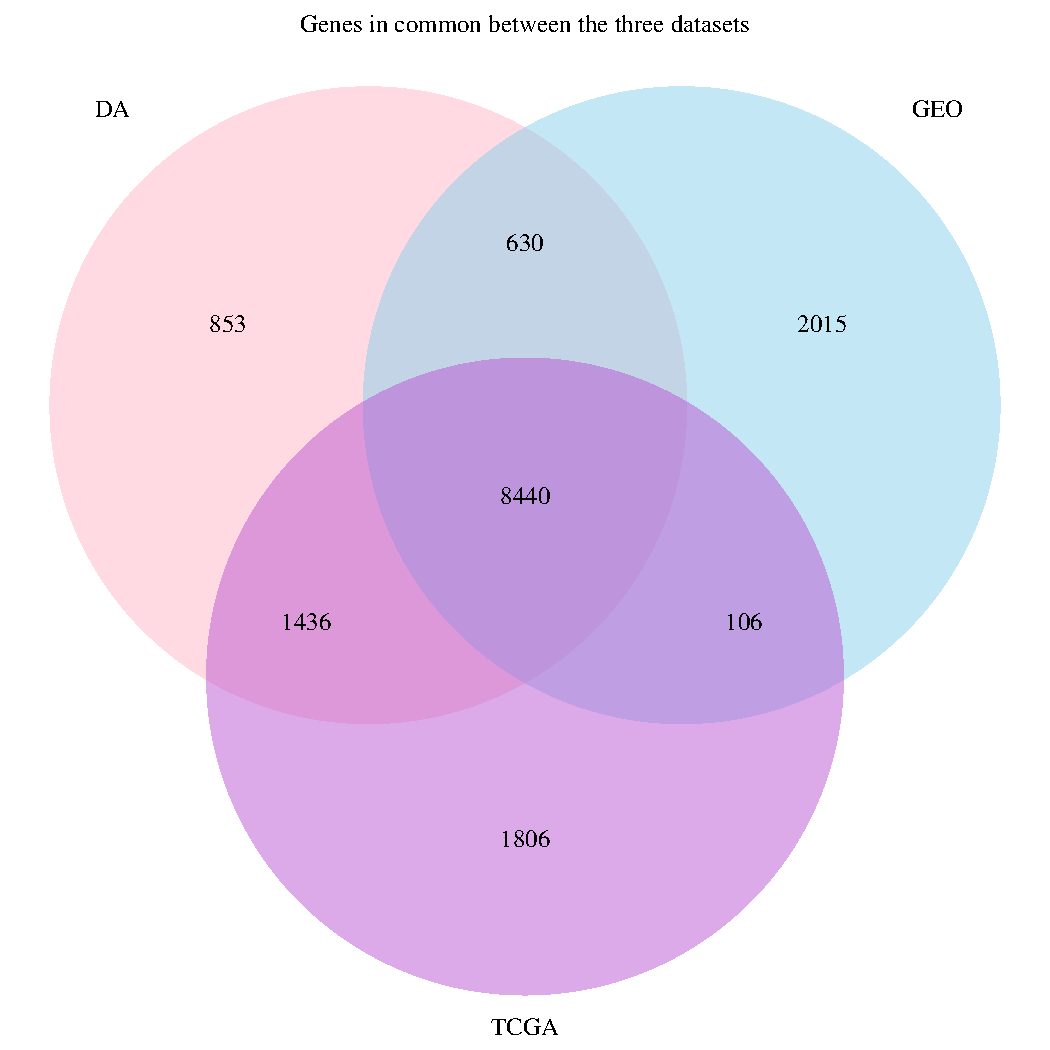
\includegraphics[width=\maxwidth]{figure/vennCommonGenesin3lists-1} 
\end{knitrout}

The data for these analyses must have a common structure: \textbf{Each pair of matrices (Expression-Methylation) must have the same rome and column names}, that is both datasets must contain information for the same genes and same samples at their corresponding positions.

This can be checked using a simple function such as \texttt{checkData} available in the package.
\begin{knitrout}
\definecolor{shadecolor}{rgb}{0.969, 0.969, 0.969}\color{fgcolor}\begin{kframe}
\begin{alltt}
\hlkwd{try}\hlstd{(}\hlkwa{if}\hlstd{(}\hlopt{!}\hlkwd{checkPairing}\hlstd{(DAExprData, DAMetilData))} \hlkwd{stop}\hlstd{(}\hlstr{"Row names and/or column names do not match"}\hlstd{))}
\hlkwd{try}\hlstd{(}\hlkwa{if}\hlstd{(}\hlopt{!}\hlkwd{checkPairing}\hlstd{(geoExprData, geoMetilData))} \hlkwd{stop}\hlstd{(}\hlstr{"Row names and/or column names do not match"}\hlstd{))}
\end{alltt}
\end{kframe}
\end{knitrout}

When one is studying the relation between methylation and expression for a bunch of genes it may be convenient to (be able) to plot the scatterplots depicting the relation between these variables. Function \texttt{plotGenesMat} allows to draw such plots.

Some examples of using this function with the first four genes of the TCGA dataset are shown below. 

\begin{figure}
\begin{knitrout}
\definecolor{shadecolor}{rgb}{0.969, 0.969, 0.969}\color{fgcolor}
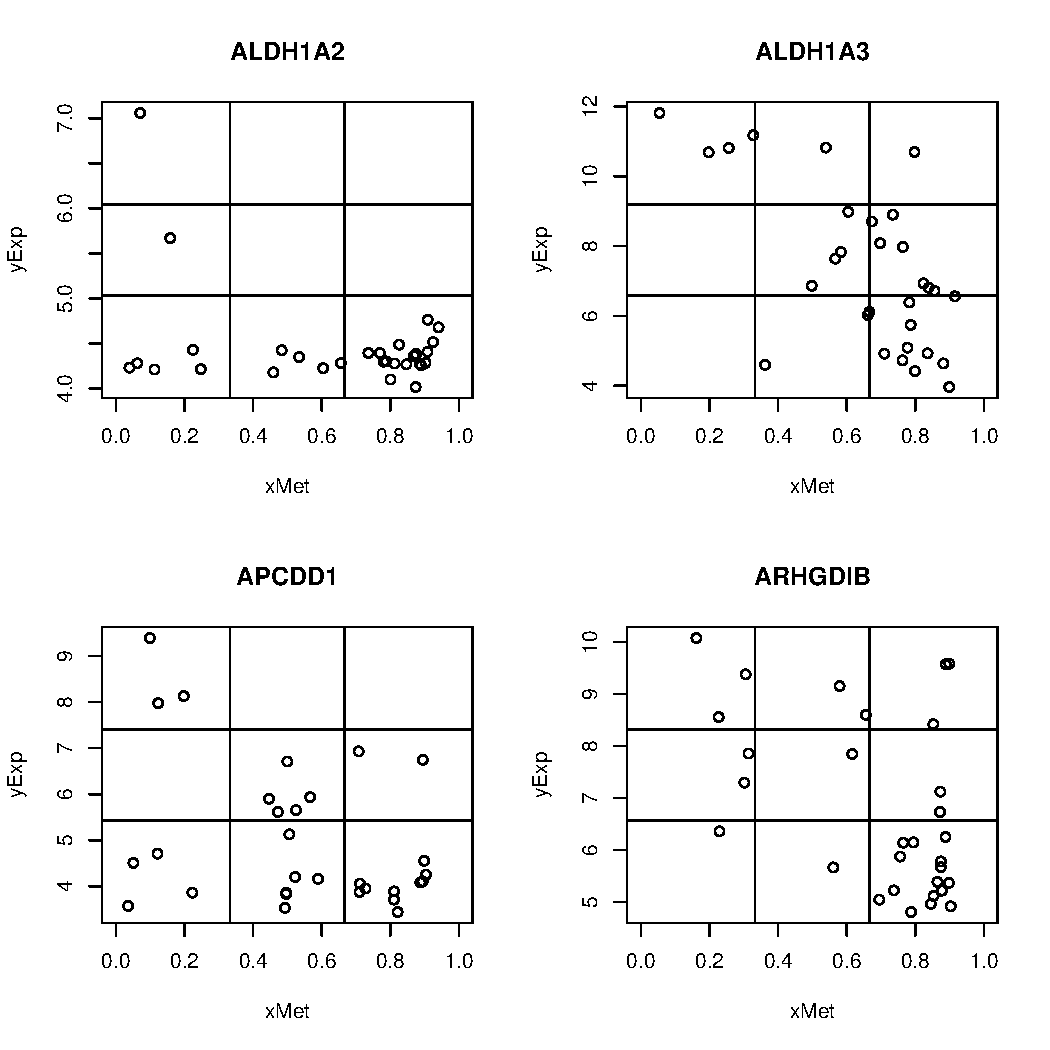
\includegraphics[width=\maxwidth]{figure/plot4Genes1-1} 
\end{knitrout}
\caption{"Scatter plot of first four genes in DA dataset (microarrays)"\label{plot4Genes1}}
\end{figure}


\begin{figure}
\begin{knitrout}
\definecolor{shadecolor}{rgb}{0.969, 0.969, 0.969}\color{fgcolor}
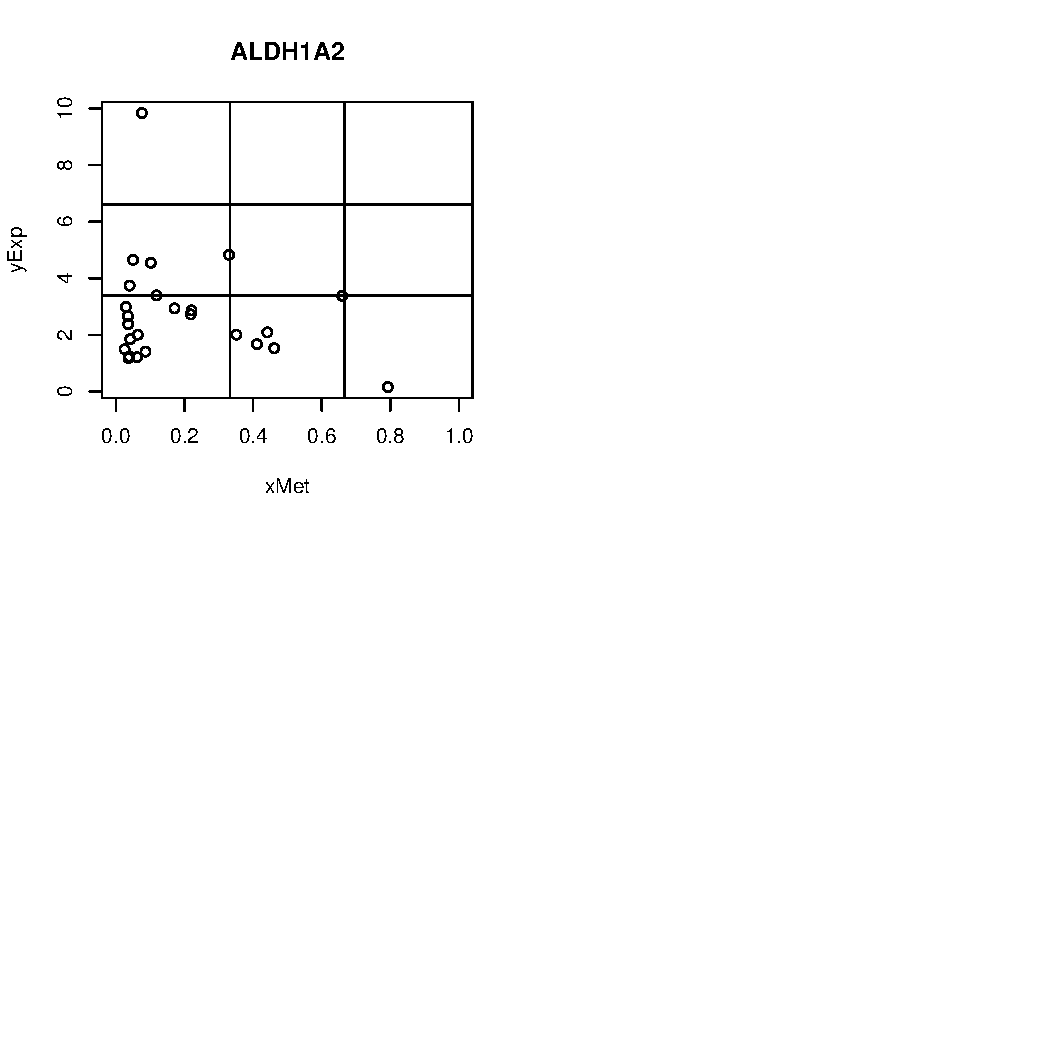
\includegraphics[width=\maxwidth]{figure/plot4Genes3-1} 
\end{knitrout}
\caption{"Scatter plot of first four genes in GEO dataset (microarrays)"\label{plot4Genes3}}
\end{figure}

\begin{figure}
\begin{knitrout}
\definecolor{shadecolor}{rgb}{0.969, 0.969, 0.969}\color{fgcolor}
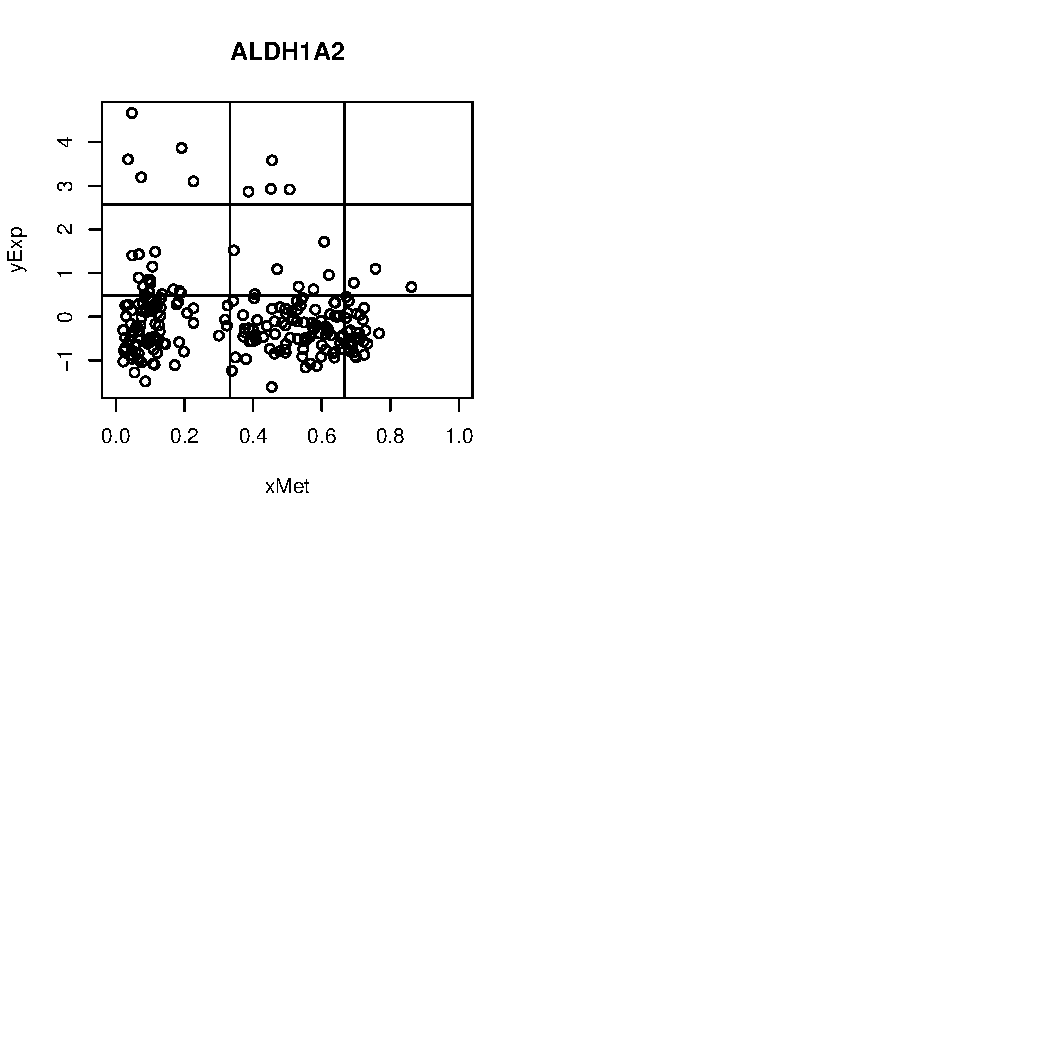
\includegraphics[width=\maxwidth]{figure/plot4Genes4-1} 
\end{knitrout}
\caption{"Scatter plot of first four genes in TCGA dataset (microarrays)"\label{plot4Genes4}}
\end{figure}

Looking at figures \ref{plot4Genes2}, \ref{plot4Genes3}, \ref{plot4Genes4} shows that although the genes may behave similarly  between datasets methods for selecting GRM must be robust and adaptable to for eample distinct sample sizes.

\subsubsection{Gene ZBTB18}

Figure \ref{plotZBTB18} shows how the scatterplot looks like for a gene that has been described bu the researchers as regulated by methylation

\begin{figure}
\begin{knitrout}
\definecolor{shadecolor}{rgb}{0.969, 0.969, 0.969}\color{fgcolor}
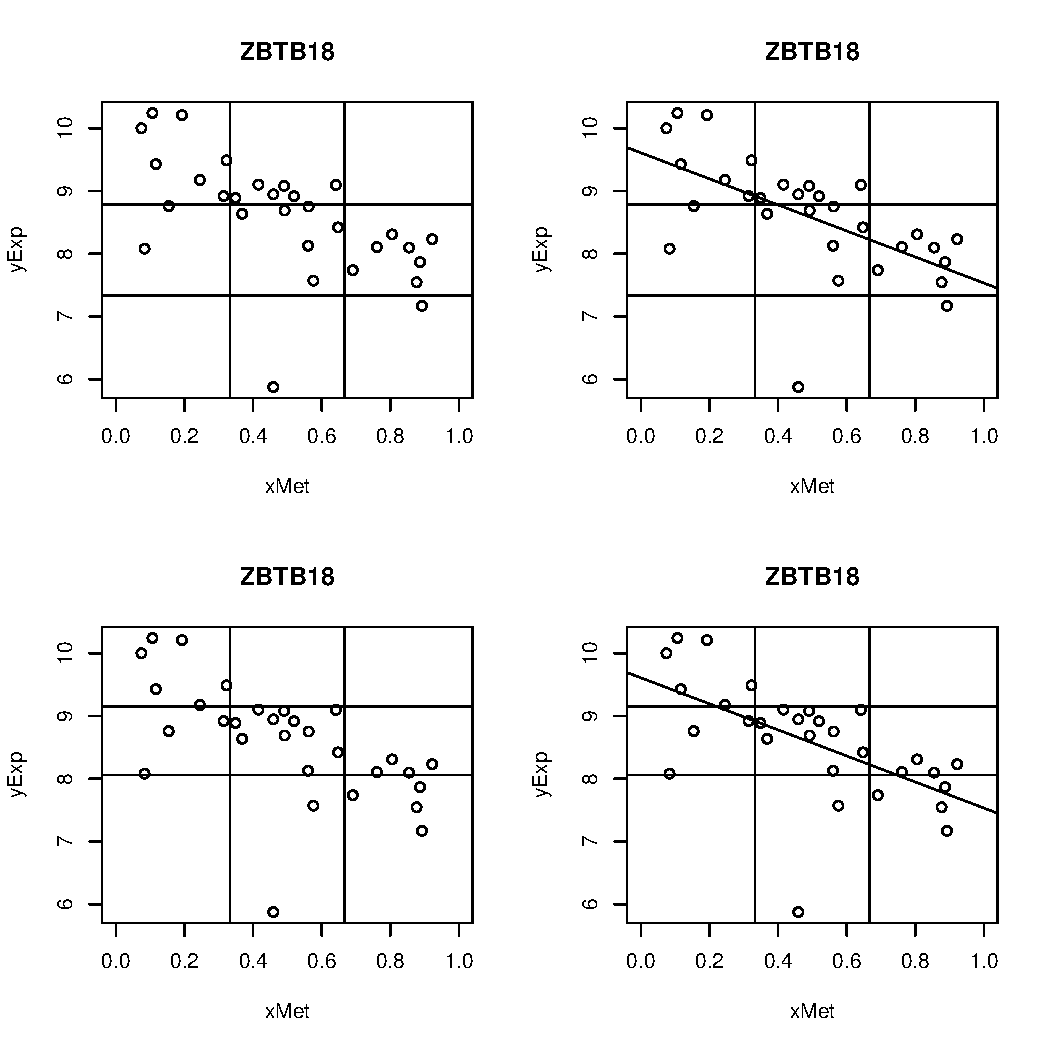
\includegraphics[width=\maxwidth]{figure/plotZBTB18-1} 
\end{knitrout}
\caption{"Scatter plot of gene ZBTB18. It seems clear that this gene will be selected by a method that selects genes negatively correlated rather than "L-shaped", although the grid could be adequately tuned for selecting it as shown in the plot."\label{plotZBTB18}}
\end{figure}


\subsection{Artificial TRUE and FALSE L-shaped genes}

\subsubsection{Genes extracted from DA dataset}

Two small sets of genes\footnote{TRUE and FALSE genes from the original dataset `` DA'' have been obtained by doing an extensive  sampling on the original dataset and selecting genes that \emph{seemed} to have an L-shape and those that did not} have been compiled with genes that were clearly L-shaped or clearly non-L-Shaped. Because these sets have been prepared arbitrarily we decide not to use them as "TRUE POSITIVE" and "TRUE NEGATIVES" except for illustrative purposes.

\begin{knitrout}
\definecolor{shadecolor}{rgb}{0.969, 0.969, 0.969}\color{fgcolor}\begin{kframe}
\begin{alltt}
\hlcom{## Genes True i False}
\hlstd{trueLGeneDF} \hlkwb{<-}\hlkwd{read.table}\hlstd{(}\hlkwd{file.path}\hlstd{(dadesDir,} \hlstr{"genesTrueLNEW.txt"}\hlstd{))}
\hlstd{(trueLGeneNames} \hlkwb{<-} \hlkwd{as.character}\hlstd{(trueLGeneDF[,}\hlnum{1}\hlstd{]))}
\end{alltt}
\begin{verbatim}
##  [1] "ABCG2"      "ADH6"       "AKR1C4"     "BCL11B"     "CA9"       
##  [6] "CCR6"       "CST7"       "CX3CL1"     "DAPP1"      "CYP27A1"   
## [11] "ELAVL2"     "FAM84A"     "GREM1"      "HSD17B2"    "INHBB"     
## [16] "KCNV1"      "LHFP"       "MEP1A"      "LRP2"       "MAGEE1"    
## [21] "MEP1A"      "MYT1"       "NOX1"       "OAS2"       "PHYHIPL"   
## [26] "POF1B"      "POPDC3"     "PRDM16"     "PRDM5"      "QPCT"      
## [31] "RASGRF2"    "RAB6B"      "RASEF"      "RNF186"     "SOX2"      
## [36] "SOSTDC1"    "SPON1"      "ST6GALNAC1" "STEAP4"     "STK33"     
## [41] "TAPBPL"     "SYN2"       "THRB"       "TRAM1L1"    "WNK4"
\end{verbatim}
\begin{alltt}
\hlstd{falseLGeneDF} \hlkwb{<-} \hlkwd{read.table}\hlstd{(}\hlkwd{file.path}\hlstd{(dadesDir,} \hlstr{"genesFalseLNEW.txt"}\hlstd{))}
\hlstd{(falseLGeneNames} \hlkwb{<-} \hlkwd{as.character}\hlstd{(falseLGeneDF[,}\hlnum{1}\hlstd{]))}
\end{alltt}
\begin{verbatim}
##  [1] "ACOX2"     "ADA"       "AKR1B1"    "ALDH1A3"   "AMT"       "ANXA3"    
##  [7] "ARHGAP4"   "ARL14"     "ATP6AP2"   "AUTS2"     "BHLHB9"    "BMP7"     
## [13] "C19orf33"  "C1QTNF6"   "CAB39L"    "CDH17"     "CDX1"      "CFTR"     
## [19] "CIDEB"     "CMTM3"     "DNAJA4"    "DUSP9"     "ELF3"      "ELMO3"    
## [25] "FBP1"      "FGD4"      "FKBP10"    "FOXC1"     "FUCA2"     "GNG4"     
## [31] "GPRC5A"    "GRAMD3"    "H1F0"      "HIST1H2BH" "HNMT"      "HOOK1"    
## [37] "HOOK3"     "HOXB3"     "HOXB2"     "HOXB5"     "HS3ST1"    "LCMT2"    
## [43] "LAMA3"     "LDHB"
\end{verbatim}
\begin{alltt}
\hlstd{trueLExpr} \hlkwb{<-} \hlstd{DAExprData[}\hlkwd{rownames}\hlstd{(DAExprData)} \hlopt \hlstd{trueLGeneNames ,]}
\hlstd{falseLExpr} \hlkwb{<-} \hlstd{DAExprData[}\hlkwd{rownames}\hlstd{(DAExprData)} \hlopt \hlstd{falseLGeneNames ,]}
\hlstd{trueLMet} \hlkwb{<-} \hlstd{DAMetilData[}\hlkwd{rownames}\hlstd{(DAMetilData)} \hlopt \hlstd{trueLGeneNames ,]}
\hlstd{falseLMet} \hlkwb{<-} \hlstd{DAMetilData[}\hlkwd{rownames}\hlstd{(DAMetilData)} \hlopt \hlstd{falseLGeneNames ,]}
\hlkwa{if}\hlstd{(}\hlopt{!}\hlstd{(}\hlkwd{file.exists}\hlstd{(}\hlstr{"DATrueLExpression.csv"}\hlstd{)))}
    \hlkwd{write.table}\hlstd{(trueLExpr,} \hlkwd{file.path}\hlstd{(dadesDir,} \hlstr{"DATrueLExpression.csv"}\hlstd{),}
                \hlkwc{sep}\hlstd{=}\hlstr{";"}\hlstd{,} \hlkwc{dec}\hlstd{=}\hlstr{"."}\hlstd{,} \hlkwc{quote}\hlstd{=}\hlnum{FALSE}\hlstd{)}
\hlkwa{if}\hlstd{(}\hlopt{!}\hlstd{(}\hlkwd{file.exists}\hlstd{(}\hlstr{"DATrueLMetilacion.csv"}\hlstd{)))}
    \hlkwd{write.table}\hlstd{(trueLMet,} \hlkwd{file.path}\hlstd{(dadesDir,} \hlstr{"DATrueLMetilacion.csv"}\hlstd{),}
                \hlkwc{sep}\hlstd{=}\hlstr{";"}\hlstd{,} \hlkwc{dec}\hlstd{=}\hlstr{"."}\hlstd{,} \hlkwc{quote}\hlstd{=}\hlnum{FALSE}\hlstd{)}
    \hlcom{# tt<- read.table(file.path(dadesDir, "DATrueLMetilacion.csv"), sep=";", dec=".")}
\end{alltt}
\end{kframe}
\end{knitrout}

Figures \ref{Lshaped1} and \ref{Lshaped2} show the first four genes of each type for illustrative purposes.

\begin{figure}
\centering
\begin{knitrout}
\definecolor{shadecolor}{rgb}{0.969, 0.969, 0.969}\color{fgcolor}\begin{kframe}
\begin{alltt}
\hlstd{opt}\hlkwb{<-} \hlkwd{par}\hlstd{(}\hlkwc{mfrow}\hlstd{=}\hlkwd{c}\hlstd{(}\hlnum{2}\hlstd{,}\hlnum{2}\hlstd{))}
\hlkwd{plotGenesMat} \hlstd{(}\hlkwc{mets}\hlstd{=trueLMet[}\hlnum{1}\hlopt{:}\hlnum{4}\hlstd{,],} \hlkwc{expres}\hlstd{=trueLExpr[}\hlnum{1}\hlopt{:}\hlnum{4}\hlstd{,],}
              \hlkwc{x1}\hlstd{=}\hlnum{1}\hlopt{/}\hlnum{3}\hlstd{,} \hlkwc{x2}\hlstd{=}\hlnum{2}\hlopt{/}\hlnum{3}\hlstd{,} \hlkwc{percY1}\hlstd{=}\hlnum{1}\hlopt{/}\hlnum{3}\hlstd{,} \hlkwc{percY2}\hlstd{=}\hlnum{2}\hlopt{/}\hlnum{3}\hlstd{,}
              \hlkwc{fileName}\hlstd{=}\hlkwa{NULL}\hlstd{,} \hlkwc{plotGrid} \hlstd{=} \hlnum{TRUE}\hlstd{)}
\hlkwd{par}\hlstd{(opt)}
\end{alltt}
\end{kframe}
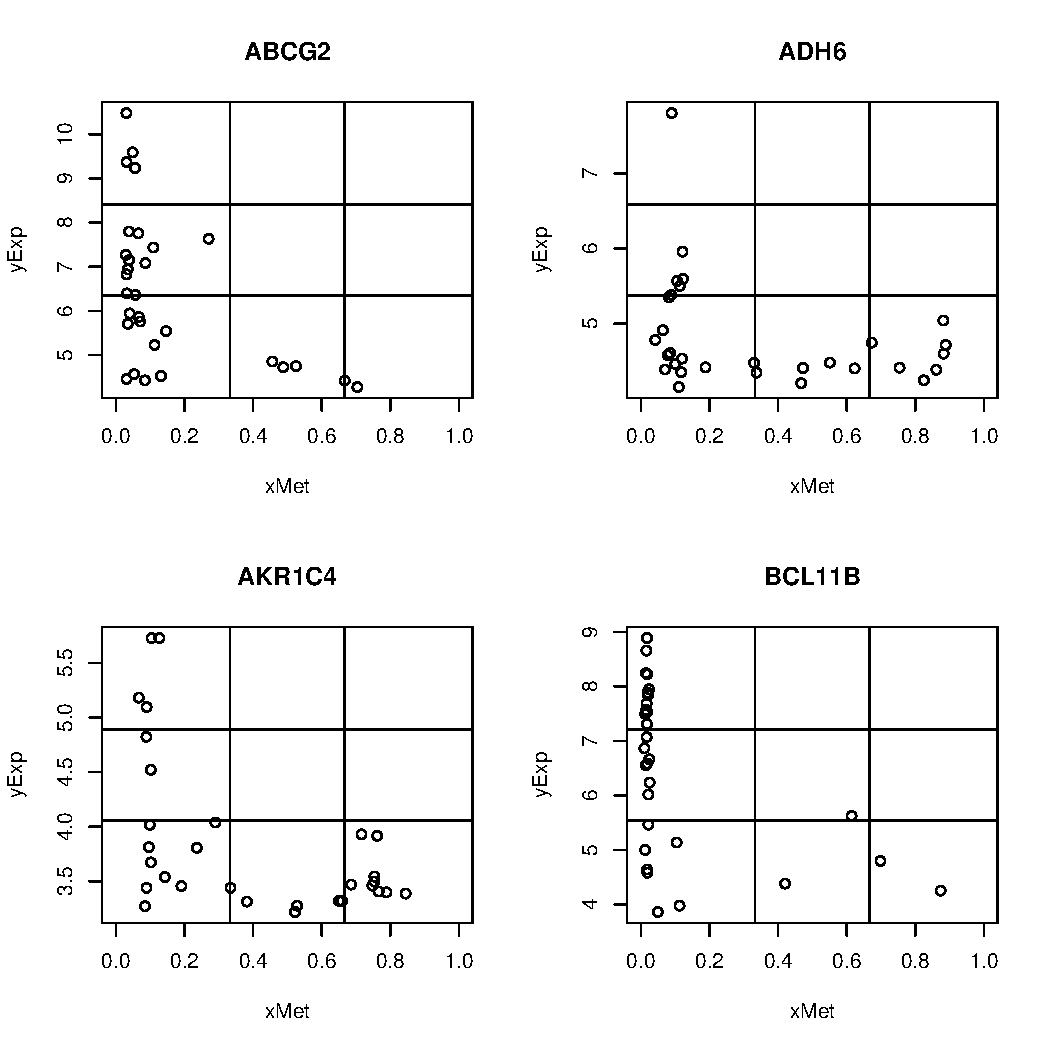
\includegraphics[width=\maxwidth]{figure/plotTRUE1-1} 
\end{knitrout}
\caption{Example of ``True'' L-shaped genes\label{Lshaped1}}
\end{figure}opt<- par(mfrow=c(2,2))


\begin{figure}
\centering
\begin{knitrout}
\definecolor{shadecolor}{rgb}{0.969, 0.969, 0.969}\color{fgcolor}\begin{kframe}
\begin{alltt}
\hlstd{opt}\hlkwb{<-} \hlkwd{par}\hlstd{(}\hlkwc{mfrow}\hlstd{=}\hlkwd{c}\hlstd{(}\hlnum{2}\hlstd{,}\hlnum{2}\hlstd{))}
\hlkwd{plotGenesMat} \hlstd{(}\hlkwc{mets}\hlstd{=falseLMet[}\hlnum{1}\hlopt{:}\hlnum{4}\hlstd{,],} \hlkwc{expres}\hlstd{=falseLExpr[}\hlnum{1}\hlopt{:}\hlnum{4}\hlstd{,],}
              \hlkwc{x1}\hlstd{=}\hlnum{1}\hlopt{/}\hlnum{3}\hlstd{,} \hlkwc{x2}\hlstd{=}\hlnum{2}\hlopt{/}\hlnum{3}\hlstd{,} \hlkwc{percY1}\hlstd{=}\hlnum{1}\hlopt{/}\hlnum{3}\hlstd{,} \hlkwc{percY2}\hlstd{=}\hlnum{2}\hlopt{/}\hlnum{3}\hlstd{,}
               \hlkwc{fileName}\hlstd{=}\hlkwa{NULL}\hlstd{,} \hlkwc{plotGrid} \hlstd{=} \hlnum{TRUE}\hlstd{)}
\hlkwd{par}\hlstd{(opt)}
\end{alltt}
\end{kframe}
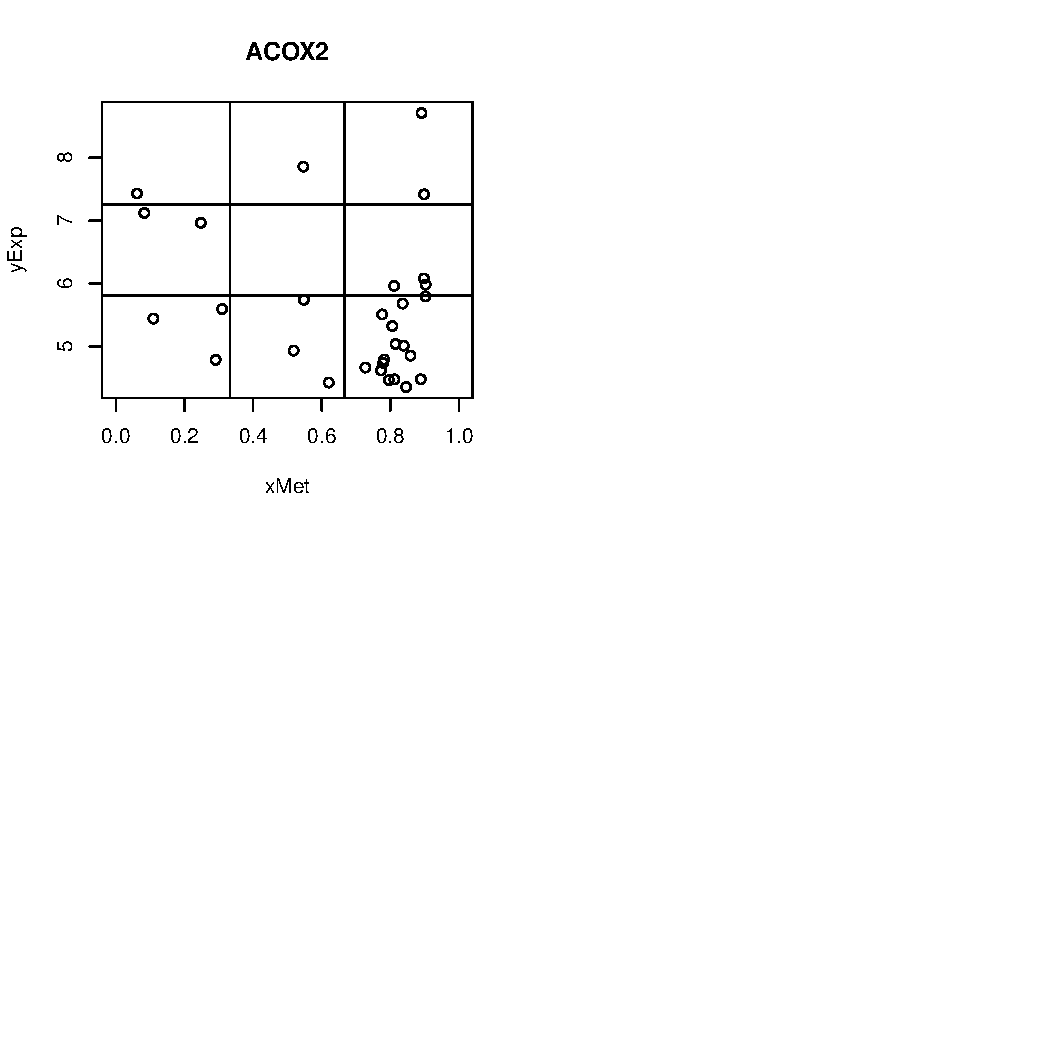
\includegraphics[width=\maxwidth]{figure/plotFALSE1-1} 
\end{knitrout}
\caption{Example of ``True'' NON-L-shaped genes\label{Lshaped2}}
\end{figure}

\subsubsection{GEO's TRUE and FALSE L-shaped genes list}

Similarly to what we have done with the researcher's dataset we have \textbf{visually} selected a set of L-shaped genes Two small sets of genes have been compiled with genes that were clearly L-shaped or clearly non-L-Shaped. Because these sets have been prepared arbitrarily we decide not to use them as "TRUE POSITIVE" and "TRUE NEGATIVES" except for illustrative purposes.

\begin{knitrout}
\definecolor{shadecolor}{rgb}{0.969, 0.969, 0.969}\color{fgcolor}\begin{kframe}
\begin{alltt}
\hlcom{## Genes True i False}
\hlstd{GEOTrueFalse} \hlkwb{<-} \hlkwd{read.table}\hlstd{(}\hlkwd{file.path}\hlstd{(dadesDir,} \hlstr{"GEOTrueFalse.txt"}\hlstd{))}
\hlstd{(GEOtrueLGeneNames} \hlkwb{<-} \hlkwd{as.character}\hlstd{(GEOTrueFalse[GEOTrueFalse[,}\hlnum{2}\hlstd{]}\hlopt{!=}\hlnum{0}\hlstd{,}\hlnum{1}\hlstd{]))}
\end{alltt}
\begin{verbatim}
##  [1] "Gene"     "LRRTM1"   "P8"       "B4GALT6"  "C1QL1"    "CNR1"    
##  [7] "DMBT1"    "ELOVL6"   "EOMES"    "ERG"      "GSTM3"    "IL17RC"  
## [13] "LPHN2"    "MME"      "MMP19"    "MOSPD2"   "MSX2"     "MTCP1"   
## [19] "MTMR8"    "NCOR2"    "P4HA3"    "SH3GL2"   "SMARCA1"  "SMO"     
## [25] "TITF1"    "TLR7"     "TP53INP1" "TRPM8"    "UBL4A"    "ZNF550"  
## [31] "ZNF71"
\end{verbatim}
\begin{alltt}
\hlstd{(GEOfalseLGeneNames} \hlkwb{<-} \hlkwd{as.character}\hlstd{(GEOTrueFalse[GEOTrueFalse[,}\hlnum{2}\hlstd{]}\hlopt{==}\hlnum{0}\hlstd{,}\hlnum{1}\hlstd{]))}
\end{alltt}
\begin{verbatim}
##  [1] "KLHL20"    "PPM2C"     "SNX27"     "C6orf114"  "IMMP2L"    "NOL3"     
##  [7] "P15RS"     "PCGF2"     "NCOA2"     "PQLC2"     "SLC20A1"   "AQP9"     
## [13] "KIT"       "AP4B1"     "FOXO1A"    "C1orf102"  "NSD1"      "ANKRD23"  
## [19] "MCL1"      "SPATA21"   "C6orf72"   "ATP2A1"    "EGLN1"     "TFAP2E"   
## [25] "TMC6"      "KRTHA4"    "CHST8"     "SKI"       "MCART1"    "MYBPC3"   
## [31] "ZNF542"    "ICT1"      "RALBP1"    "SPINK5"    "IL10RB"    "BTBD10"   
## [37] "TMTC3"     "WNT3"      "C1orf142"  "MX2"       "DDX19A"    "BXDC5"    
## [43] "SIX6"      "COG1"      "ALPPL2"    "TNFRSF4"   "FLJ45983"  "IFT80"    
## [49] "LOC388407" "TIGD1"     "NKX6-2"    "PARD3"     "SYT3"      "FOXB1"    
## [55] "FLJ90166"  "EMR2"      "ABCB10"    "NDUFA4"    "TLOC1"     "SLC14A1"  
## [61] "DDX3X"     "TACC2"     "PLEKHA8"   "SP6"       "EPB41L1"   "ASB6"     
## [67] "LY6G6C"    "LRP6"      "GPR30"     "GPR1"
\end{verbatim}
\begin{alltt}
\hlstd{GEOtrueLExpr} \hlkwb{<-} \hlstd{geoExprData[}\hlkwd{rownames}\hlstd{(geoExprData)} \hlopt \hlstd{GEOtrueLGeneNames ,]}
\hlstd{GEOfalseLExpr} \hlkwb{<-} \hlstd{geoExprData[}\hlkwd{rownames}\hlstd{(geoExprData)} \hlopt \hlstd{GEOfalseLGeneNames ,]}
\hlstd{GEOtrueLMet} \hlkwb{<-} \hlstd{geoMetilData[}\hlkwd{rownames}\hlstd{(geoMetilData)} \hlopt \hlstd{GEOtrueLGeneNames ,]}
\hlstd{GEOfalseLMet} \hlkwb{<-} \hlstd{geoMetilData[}\hlkwd{rownames}\hlstd{(geoMetilData)} \hlopt \hlstd{GEOfalseLGeneNames ,]}
\hlstd{GEOTrueFalseExpr} \hlkwb{<-} \hlstd{geoExprData[}\hlkwd{rownames}\hlstd{(geoExprData)} \hlopt \hlkwd{c}\hlstd{(GEOtrueLGeneNames,GEOfalseLGeneNames) ,]}
\hlstd{GEOTrueFalseMet} \hlkwb{<-} \hlstd{geoMetilData[}\hlkwd{rownames}\hlstd{(geoMetilData)} \hlopt \hlkwd{c}\hlstd{(GEOtrueLGeneNames,GEOfalseLGeneNames) ,]}
\hlkwa{if}\hlstd{(}\hlopt{!}\hlstd{(}\hlkwd{file.exists}\hlstd{(}\hlstr{"GEOTrueLExpression.csv"}\hlstd{)))}
    \hlkwd{write.table}\hlstd{(GEOtrueLExpr,} \hlkwd{file.path}\hlstd{(dadesDir,} \hlstr{"GEOTrueLExpression.csv"}\hlstd{),}
                \hlkwc{sep}\hlstd{=}\hlstr{";"}\hlstd{,} \hlkwc{dec}\hlstd{=}\hlstr{"."}\hlstd{,} \hlkwc{quote}\hlstd{=}\hlnum{FALSE}\hlstd{)}
\hlkwa{if}\hlstd{(}\hlopt{!}\hlstd{(}\hlkwd{file.exists}\hlstd{(}\hlstr{"GEOTrueLMetilacion.csv"}\hlstd{)))}
    \hlkwd{write.table}\hlstd{(GEOtrueLMet,} \hlkwd{file.path}\hlstd{(dadesDir,} \hlstr{"GEOTrueLMetilacion.csv"}\hlstd{),}
                \hlkwc{sep}\hlstd{=}\hlstr{";"}\hlstd{,} \hlkwc{dec}\hlstd{=}\hlstr{"."}\hlstd{,} \hlkwc{quote}\hlstd{=}\hlnum{FALSE}\hlstd{)}
    \hlcom{# tt<- read.table(file.path(dadesDir, "GEOTrueLMetilacion.csv"), sep=";", dec="."); head(tt)}
\end{alltt}
\end{kframe}
\end{knitrout}

Figures \ref{GEOLshaped1} and \ref{GEOLshaped2} show the first four genes of each type for illustrative purposes.

\begin{figure}
\centering
\begin{knitrout}
\definecolor{shadecolor}{rgb}{0.969, 0.969, 0.969}\color{fgcolor}\begin{kframe}
\begin{alltt}
\hlstd{opt}\hlkwb{<-} \hlkwd{par}\hlstd{(}\hlkwc{mfrow}\hlstd{=}\hlkwd{c}\hlstd{(}\hlnum{2}\hlstd{,}\hlnum{2}\hlstd{))}
\hlkwd{plotGenesMat} \hlstd{(}\hlkwc{mets}\hlstd{=GEOtrueLMet[}\hlnum{1}\hlopt{:}\hlnum{4}\hlstd{,],} \hlkwc{expres}\hlstd{=GEOtrueLExpr[}\hlnum{1}\hlopt{:}\hlnum{4}\hlstd{,],}
               \hlkwc{fileName}\hlstd{=}\hlkwa{NULL}\hlstd{,} \hlkwc{plotGrid} \hlstd{=} \hlnum{TRUE}\hlstd{)}
\hlkwd{par}\hlstd{(opt)}
\end{alltt}
\end{kframe}
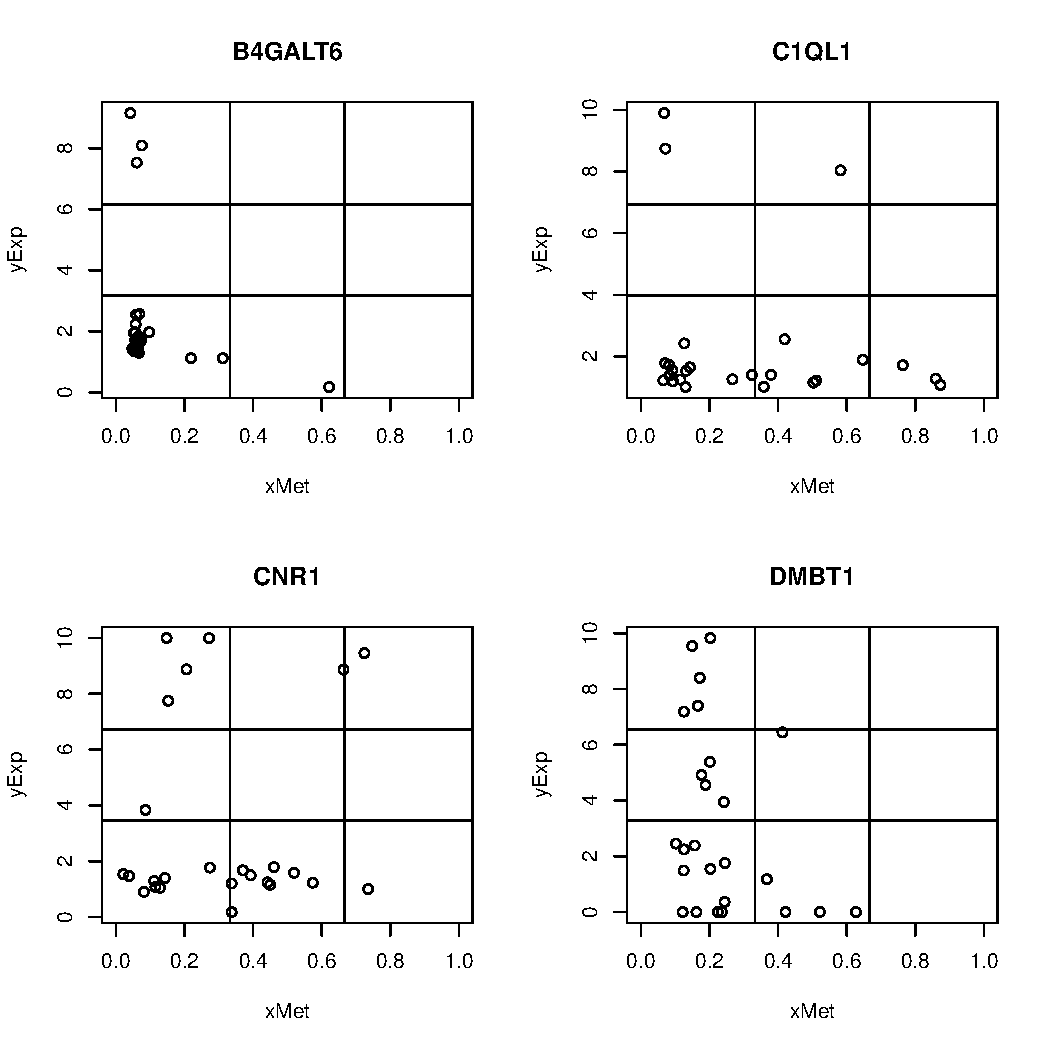
\includegraphics[width=\maxwidth]{figure/plotTRUE2-1} 
\end{knitrout}
\caption{Example of ``True'' L-shaped genes\label{Lshaped12}}
\end{figure}opt<- par(mfrow=c(2,2))


\begin{figure}
\centering
\begin{knitrout}
\definecolor{shadecolor}{rgb}{0.969, 0.969, 0.969}\color{fgcolor}\begin{kframe}
\begin{alltt}
\hlstd{opt}\hlkwb{<-} \hlkwd{par}\hlstd{(}\hlkwc{mfrow}\hlstd{=}\hlkwd{c}\hlstd{(}\hlnum{2}\hlstd{,}\hlnum{2}\hlstd{))}
\hlkwd{plotGenesMat} \hlstd{(}\hlkwc{mets}\hlstd{=GEOfalseLMet[}\hlnum{1}\hlopt{:}\hlnum{4}\hlstd{,],} \hlkwc{expres}\hlstd{=GEOfalseLExpr[}\hlnum{1}\hlopt{:}\hlnum{4}\hlstd{,],}
              \hlkwc{x1}\hlstd{=}\hlnum{1}\hlopt{/}\hlnum{3}\hlstd{,} \hlkwc{x2}\hlstd{=}\hlnum{2}\hlopt{/}\hlnum{3}\hlstd{,} \hlkwc{y1}\hlstd{=y1,} \hlkwc{y2}\hlstd{=y2,}
               \hlkwc{fileName}\hlstd{=}\hlkwa{NULL}\hlstd{,} \hlkwc{plotGrid} \hlstd{=} \hlnum{TRUE}\hlstd{)}
\hlkwd{par}\hlstd{(opt)}
\end{alltt}
\end{kframe}
\end{knitrout}
\caption{Example of ``True'' NON-L-shaped genes\label{Lshaped2}}
\end{figure}


\section{Scoring scatterplots}

\subsection{The ``three band rule''}

After trying different approaches to detect L-shapes, one often comes back to a naive approach like \emph{``L-shaped'' genes should show an L shape in the scatterplot, that is, values should tend to be scattered near the vertical and horizontal axes, and the more we move from these positions the least L-shaped the gene should be}.

This idea can be made more explicit by introducing a ``three-band rule'' as follows:
\begin{enumerate}
\item Overimpose a $3\times 3$ grid on the scatterplot.
\item Classify the scatterplot as \textbf{``L'' or ``non-L''} based on a small set of conditions:
\begin{enumerate}
  \item There must be a \emph{minimum} number of points in the upper-left (cell (1,1)) and lower right (cell (3,3)) corners of the grid.
  \item There must be a \emph{maximum} number of points in the upper right (cell (1,3)) because points there mean hypermethylation and hyperexpression which is the opposite of what we are looking for.
  \item We will usually \emph{not require to have a minimum of points in cell (3,1)} unless we are really willing to have an L-shape (in our setting we will also be happy tho recover diagonals, which also reflect a negative correlation!).
\end{enumerate}

\item Score points on each subgrid in such a way that
\begin{enumerate}
	\item Points in permitted regions (left-outer margin, i.e. cells: (1,1), (2,2), (3,1), (3,2), (3,3)) score positively if the scatterplot has been classified as L or zero if it has been classified as non-L.
	\item Points in non-desired regions (outer band. i.e. cells (1,2), (1,3), (2,3)) score negatively in all cases.
	\item Some regions may be declared neutral and not-score, such as cell (2,2).
\end{enumerate}
\item Use cross-validation to tune scoring parameters (\textbf{if a set of positive and negative L-shaped genes is available}).
\end{enumerate}

The previous scheme can be summarized using the following equation.
\begin{equation}
S(X) = W_L \circ X \times \mathbbm{1}_L(X) + W_{L^C} \circ X \times \mathbbm{1}_{L^c}(X),
\end{equation}
where
\begin{itemize}
\item ${X}$ is the matrix of \emph{counts}, i.e. the number of counts in each cell of the grid,
\item ${W_L}$ is the matrix of scores per cell and point \emph{if the scatterplot has been classified as $L$},
\item ${W_{L^c}}$ is the matrix of scores per cell and point \emph{if the scatterplot has been classified as non-$L$ ($L^c$)},
\end{itemize}
and $\circ$ represents the hadamard product of the two matrices $W_{L/L^c}$ (i.e. elementwise multiplication of the two matrices) and $\mathbbm{1}_{L/L^c}()$ is the indicator function for $L$ or $L^c$.

The fact that the scatterplot is assigned to $L$ or $L^c$ can also be described as the hadamard product of three matrices:
\begin{equation}
\mathbbm{1}_L(X) = \bigwedge_{i,j} X \circ C \circ \left( mMP \times \sum_{i,j}x_{ij}\right),
\end{equation}
where 
\begin{itemize}
\item ${X}$ is the matrix of \emph{counts}, i.e. the number of counts in each cell of the grid,
\item $C$ is the matrix of conditions to be verified \emph{if the scatterplot has to be classified as $L$},
\item $mMP$ is the matrix of minimum and Maximum Percentages of points to have in each cell \emph{if the scatterplot has to be classified as $L$},
\item $\circ$ represents the pointwise logical operation which allows that the product of the three cells becomes a logical operation and
\item $\bigwedge_{i,j}$ represents an logical ``AND'' operation of all cells, that is if all cells are TRUE the result is assigned to $L$ and if one fails it is assigned to $L^c$.
\end{itemize}

This idea is summarized in figure \ref{Lscore}
\begin{figure}[htbp]
\centering
	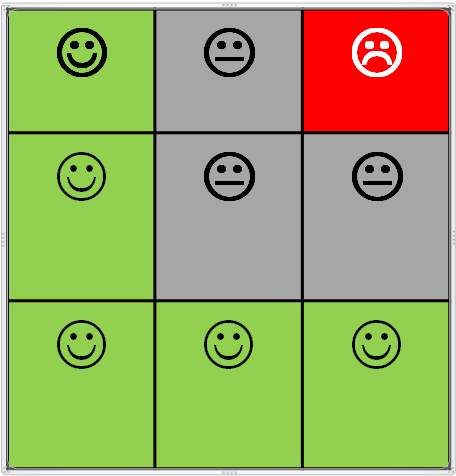
\includegraphics[width=0.7\textwidth]{./images/Lscoring.png}
\caption{The heuristic method is based in scoring differently depending on where the points are found on a grid\label{Lscore}}
\end{figure}


\subsection{Computing on a grid}

We have developed several functions to help detect and select L--shape scatterplots.
Their use is described in the package help but they are illustrated here to clarify the code below.

\begin{itemize}
\item \texttt{calcFreqs} counts the number of points in each cell of the grid for given vertical (defined by parameters \texttt{x1}, \texttt{x2}) and horizontal lines (defined by parameters \texttt{y1}, \texttt{y2}, \texttt{percY1}, \texttt{percY2}) 
\item \texttt{binScore} classifies (\emph{scores binarily}) a scatterplot based on the rules described above, that is it checks if the minimal assumptions for an L-shape hold or not. It needs a matrix of \emph{min-max frequency counts}.
\item \texttt{numScore} scores a scatterplot using a matrix of weights that defines the score given to each point depending on the cell where it is located. 
\begin{itemize}
  \item If the scatterplot has been classified as having L-shape all points are scored, those in favorable regions score positively and those in non-favorable regions negatively. 
  \item If the scatterplot has not been classifed as "L" only points in non-favourable regions score negatively. 
\end{itemize}
\item \texttt{scoreGenesMat} is a wrapper for scoring the genes provided in two related matrices that is, it first applies the \texttt{binScore} function and depending on its results it computes the \texttt{numericScore} function with all the genes in the (pair of) matrices.
\item Function \texttt{plotGenesMat} is not a computing function but it is worth to enumerate it here because it complements the other functions by allowing to visualize the data that have generated a certain score from a given scatterplot.
\end{itemize}

\subsection{Examples}

\subsubsection{Scoring the TRUE/FALSE DA dataset}

The first example below show that genes that have been marked as TRUE or FALSE L in the DA dataset \textbf{may} score different.

\begin{knitrout}
\definecolor{shadecolor}{rgb}{0.969, 0.969, 0.969}\color{fgcolor}\begin{kframe}
\begin{alltt}
\hlstd{xVecTrue}\hlkwb{<-} \hlkwd{as.numeric}\hlstd{(trueLMet[}\hlnum{1}\hlstd{,])}
\hlstd{yVecTrue}\hlkwb{<-} \hlkwd{as.numeric}\hlstd{(trueLExpr[}\hlnum{1}\hlstd{,])}
\hlstd{reqPercentages} \hlkwb{<-} \hlkwd{matrix} \hlstd{(}\hlkwd{c}\hlstd{(}\hlnum{10}\hlstd{,} \hlnum{20}\hlstd{,} \hlnum{0}\hlstd{,} \hlnum{5}\hlstd{,} \hlnum{0}\hlstd{,} \hlnum{20}\hlstd{,} \hlnum{0}\hlstd{,} \hlnum{5}\hlstd{,} \hlnum{5}\hlstd{),} \hlkwc{nrow}\hlstd{=}\hlnum{3}\hlstd{,} \hlkwc{byrow}\hlstd{=}\hlnum{TRUE}\hlstd{)}

\hlkwd{messageTitle}\hlstd{(}\hlstr{"Frequency count in first ``TRUE'' gene"}\hlstd{)}
\hlstd{(geneGridTrue} \hlkwb{<-} \hlkwd{calcFreqs}\hlstd{(}\hlkwc{xMet}\hlstd{=xVecTrue,} \hlkwc{yExp}\hlstd{=yVecTrue,} \hlkwc{x1}\hlstd{=}\hlnum{1}\hlopt{/}\hlnum{3}\hlstd{,} \hlkwc{x2}\hlstd{=}\hlnum{2}\hlopt{/}\hlnum{3}\hlstd{,}
                          \hlkwc{y1}\hlstd{=}\hlkwa{NULL}\hlstd{,} \hlkwc{y2}\hlstd{=}\hlkwa{NULL}\hlstd{,} \hlkwc{percY1}\hlstd{=}\hlnum{1}\hlopt{/}\hlnum{3}\hlstd{,} \hlkwc{percY2}\hlstd{=}\hlnum{2}\hlopt{/}\hlnum{3}\hlstd{))}
\end{alltt}
\end{kframe}


\begin{tabular}{r|r|r}
\hline
4 & 0 & 0\\
\hline
11 & 0 & 0\\
\hline
10 & 3 & 2\\
\hline
\end{tabular}\begin{kframe}\begin{alltt}
\hlstd{(maxminCountsT} \hlkwb{<-} \hlkwd{toReqMat} \hlstd{(}\hlkwd{sum}\hlstd{(geneGridTrue), reqPercentages))}
\end{alltt}
\end{kframe}


\begin{tabular}{r|r|r}
\hline
3 & 6 & 0\\
\hline
2 & 0 & 6\\
\hline
0 & 2 & 2\\
\hline
\end{tabular}\begin{kframe}\begin{alltt}
\hlstd{(aWeightMifL}\hlkwb{=}\hlkwd{matrix} \hlstd{(}\hlkwd{c}\hlstd{(}\hlnum{2}\hlstd{,}\hlopt{-}\hlnum{2}\hlstd{,}\hlopt{-}\hlnum{25}\hlstd{,}\hlnum{1}\hlstd{,}\hlnum{0}\hlstd{,}\hlopt{-}\hlnum{2}\hlstd{,}\hlnum{1}\hlstd{,}\hlnum{1}\hlstd{,}\hlnum{2}\hlstd{),} \hlkwc{nrow}\hlstd{=}\hlnum{3}\hlstd{,} \hlkwc{byrow}\hlstd{=}\hlnum{TRUE}\hlstd{))}
\end{alltt}
\end{kframe}


\begin{tabular}{r|r|r}
\hline
2 & -2 & -25\\
\hline
1 & 0 & -2\\
\hline
1 & 1 & 2\\
\hline
\end{tabular}\begin{kframe}\begin{alltt}
\hlstd{(aWeightMifNonL}\hlkwb{=}\hlkwd{matrix} \hlstd{(}\hlkwd{c}\hlstd{(}\hlnum{0}\hlstd{,}\hlopt{-}\hlnum{2}\hlstd{,}\hlopt{-}\hlnum{25}\hlstd{,}\hlnum{0}\hlstd{,}\hlnum{0}\hlstd{,}\hlopt{-}\hlnum{2}\hlstd{,}\hlnum{0}\hlstd{,}\hlnum{0}\hlstd{,}\hlnum{0}\hlstd{),} \hlkwc{nrow}\hlstd{=}\hlnum{3}\hlstd{,} \hlkwc{byrow}\hlstd{=}\hlnum{TRUE}\hlstd{))}
\end{alltt}
\end{kframe}


\begin{tabular}{r|r|r}
\hline
0 & -2 & -25\\
\hline
0 & 0 & -2\\
\hline
0 & 0 & 0\\
\hline
\end{tabular}\begin{kframe}\begin{alltt}
\hlkwd{messageTitle}\hlstd{(}\hlstr{"Binary and numeric soring in first ``TRUE'' gene"}\hlstd{)}
\hlstd{(binSc}\hlkwb{<-} \hlkwd{binScore} \hlstd{(geneGridTrue, maxminCountsT ))}
\end{alltt}
\begin{verbatim}
## [1] TRUE
\end{verbatim}
\begin{alltt}
\hlstd{(nsT}\hlkwb{<-} \hlkwd{numScore}\hlstd{(geneGridTrue,} \hlkwc{LShaped} \hlstd{= binSc, aWeightMifL, aWeightMifNonL))}
\end{alltt}
\begin{verbatim}
## [1] 36
\end{verbatim}
\end{kframe}
\end{knitrout}

\begin{knitrout}
\definecolor{shadecolor}{rgb}{0.969, 0.969, 0.969}\color{fgcolor}\begin{kframe}
\begin{alltt}
\hlstd{xVecFalse}\hlkwb{<-} \hlkwd{as.numeric}\hlstd{(falseLMet[}\hlnum{1}\hlstd{,])}
\hlstd{yVecFalse}\hlkwb{<-} \hlkwd{as.numeric}\hlstd{(falseLExpr[}\hlnum{1}\hlstd{,])}

\hlkwd{messageTitle}\hlstd{(}\hlstr{"Frequency count in first ``FALSE'' gene"}\hlstd{)}
\hlstd{(geneGridFalse} \hlkwb{<-} \hlkwd{calcFreqs}\hlstd{(}\hlkwc{xMet}\hlstd{=xVecFalse,} \hlkwc{yExp}\hlstd{=yVecFalse,} \hlkwc{x1}\hlstd{=}\hlnum{1}\hlopt{/}\hlnum{3}\hlstd{,} \hlkwc{x2}\hlstd{=}\hlnum{2}\hlopt{/}\hlnum{3}\hlstd{,}
                          \hlkwc{y1}\hlstd{=}\hlkwa{NULL}\hlstd{,} \hlkwc{y2}\hlstd{=}\hlkwa{NULL}\hlstd{,} \hlkwc{percY1}\hlstd{=}\hlnum{1}\hlopt{/}\hlnum{3}\hlstd{,} \hlkwc{percY2}\hlstd{=}\hlnum{2}\hlopt{/}\hlnum{3}\hlstd{))}
\end{alltt}
\end{kframe}


\begin{tabular}{r|r|r}
\hline
1 & 1 & 2\\
\hline
2 & 0 & 3\\
\hline
3 & 3 & 15\\
\hline
\end{tabular}\begin{kframe}\begin{alltt}
\hlstd{(maxminCountsF} \hlkwb{<-} \hlkwd{toReqMat} \hlstd{(}\hlkwd{sum}\hlstd{(geneGridFalse), reqPercentages))}
\end{alltt}
\end{kframe}


\begin{tabular}{r|r|r}
\hline
3 & 6 & 0\\
\hline
2 & 0 & 6\\
\hline
0 & 2 & 2\\
\hline
\end{tabular}\begin{kframe}\begin{alltt}
\hlcom{# Same value as maxminCountsT because it depends only on required percentages and sample size}
\hlkwd{messageTitle}\hlstd{(}\hlstr{"Binary and numeric soring in first ``FALSE'' gene"}\hlstd{)}
\hlstd{(binSc}\hlkwb{<-}\hlkwd{binScore} \hlstd{(geneGridFalse, maxminCountsF))}
\end{alltt}
\begin{verbatim}
## [1] FALSE
\end{verbatim}
\begin{alltt}
\hlstd{(nsF}\hlkwb{<-} \hlkwd{numScore}\hlstd{(geneGridFalse,} \hlkwc{LShaped} \hlstd{= binSc, aWeightMifL, aWeightMifNonL))}
\end{alltt}
\begin{verbatim}
## [1] -58
\end{verbatim}
\end{kframe}
\end{knitrout}

\begin{knitrout}
\definecolor{shadecolor}{rgb}{0.969, 0.969, 0.969}\color{fgcolor}


\begin{tabular}{r|r|r}
\hline
2 & -2 & -30\\
\hline
1 & 0 & -2\\
\hline
1 & 1 & 2\\
\hline
\end{tabular}


\begin{tabular}{r|r|r}
\hline
0 & -2 & -30\\
\hline
0 & 0 & -2\\
\hline
0 & 0 & 0\\
\hline
\end{tabular}


\begin{tabular}{r|r|r}
\hline
10 & 20 & 0\\
\hline
10 & 0 & 20\\
\hline
20 & 10 & 10\\
\hline
\end{tabular}\begin{kframe}\begin{verbatim}
## Number of scatterplots scored  :  44
## Number of L-shape scatterplots :  9
\end{verbatim}
\end{kframe}


\begin{tabular}{r|r}
\hline
FALSE & TRUE\\
\hline
35 & 9\\
\hline
\end{tabular}


\begin{tabular}{r|r|r|r|r|r|r|r|r|r|r|r}
\hline
-30 & -10 & -8 & -4 & -2 & 0 & 34 & 36 & 37 & 41 & 43 & 45\\
\hline
3 & 1 & 1 & 2 & 5 & 23 & 1 & 1 & 1 & 3 & 2 & 1\\
\hline
\end{tabular}
\end{knitrout}

\begin{knitrout}
\definecolor{shadecolor}{rgb}{0.969, 0.969, 0.969}\color{fgcolor}\begin{kframe}
\begin{verbatim}
## Number of scatterplots scored  :  44
## Number of L-shape scatterplots :  0
\end{verbatim}
\end{kframe}


\begin{tabular}{r}
\hline
FALSE\\
\hline
44\\
\hline
\end{tabular}


\begin{tabular}{r|r|r|r|r|r|r|r|r|r|r|r|r|r|r|r|r|r|r|r|r|r|r|r|r|r|r|r}
\hline
-256 & -206 & -168 & -148 & -112 & -110 & -108 & -96 & -92 & -76 & -72 & -68 & -66 & -46 & -42 & -40 & -36 & -34 & -32 & -18 & -16 & -12 & -10 & -8 & -6 & -4 & -2 & 0\\
\hline
1 & 2 & 1 & 1 & 1 & 1 & 1 & 1 & 1 & 1 & 2 & 2 & 1 & 2 & 1 & 1 & 1 & 2 & 2 & 1 & 1 & 3 & 2 & 1 & 1 & 2 & 2 & 6\\
\hline
\end{tabular}
\end{knitrout}


\section{Putting all together: Selecting L-shaped genes}

The goal of developing all these functions is being able to select L-shaped genes from a paired dataset (expression-methylation) in a way that is as flexible and as rapid and as good as possible.

Essentially the process of selecting L-shape genes consists of three steps:
\begin{enumerate}
  \item Select datasets (a pair of row-column matched matrices, one for expression and one for methylation).
  \item Set parameters:
  \begin{enumerate}
    \item Grid definition
    \item Binary Scoring 
    \item Numerical Scoring
  \end{enumerate}
 \item Score the selected data and return classificaation (scores and group) and plots for each gene.
\end{enumerate}

\subsection{Parameters selection}

As it has been shown in the examples above the functions 
may be applied sequentially to an expression-methylation pair using the 
\texttt{scoreGenesMat} function.

We have selected a different set of parameters for DA and GEO datasets than for TCGA data, because as the sample size increases it seems reasonable (necessary) to be mor permisive. Strictly speaking only required percentages have been changed, not weights.

\subsubsection{Parameters for DA and GEO datasets (small samples)}
\begin{knitrout}
\definecolor{shadecolor}{rgb}{0.969, 0.969, 0.969}\color{fgcolor}\begin{kframe}
\begin{alltt}
\hlstd{(reqPercentages}   \hlkwb{<-} \hlkwd{matrix} \hlstd{(}\hlkwd{c}\hlstd{(}\hlnum{10}\hlstd{,} \hlnum{20}\hlstd{,} \hlnum{1}\hlstd{,} \hlnum{4}\hlstd{,} \hlnum{30}\hlstd{,} \hlnum{20}\hlstd{,} \hlnum{0}\hlstd{,} \hlnum{5}\hlstd{,} \hlnum{10}\hlstd{),} \hlkwc{nrow}\hlstd{=}\hlnum{3}\hlstd{,} \hlkwc{byrow}\hlstd{=}\hlnum{TRUE}\hlstd{))}
\end{alltt}
\end{kframe}


\begin{tabular}{r|r|r}
\hline
10 & 20 & 1\\
\hline
4 & 30 & 20\\
\hline
0 & 5 & 10\\
\hline
\end{tabular}\begin{kframe}\begin{alltt}
\hlstd{(maxminCounts} \hlkwb{<-} \hlkwd{toReqMat}\hlstd{(}\hlkwd{dim}\hlstd{(DAMetilData)[}\hlnum{2}\hlstd{], reqPercentages))} \hlcom{# Informative. NOt used in calculations because it is computed within the loop}
\end{alltt}
\end{kframe}


\begin{tabular}{r|r|r}
\hline
3 & 6 & 0\\
\hline
1 & 9 & 6\\
\hline
0 & 2 & 3\\
\hline
\end{tabular}\begin{kframe}\begin{alltt}
\hlstd{(theWeightMifL}\hlkwb{=}\hlkwd{matrix} \hlstd{(}\hlkwd{c}\hlstd{(}\hlnum{2}\hlstd{,}\hlopt{-}\hlnum{2}\hlstd{,}\hlopt{-}\hlnum{25}\hlstd{,}\hlnum{1}\hlstd{,}\hlnum{0}\hlstd{,}\hlopt{-}\hlnum{2}\hlstd{,}\hlnum{1}\hlstd{,}\hlnum{1}\hlstd{,}\hlnum{2}\hlstd{),} \hlkwc{nrow}\hlstd{=}\hlnum{3}\hlstd{,} \hlkwc{byrow}\hlstd{=}\hlnum{TRUE}\hlstd{))}
\end{alltt}
\end{kframe}


\begin{tabular}{r|r|r}
\hline
2 & -2 & -25\\
\hline
1 & 0 & -2\\
\hline
1 & 1 & 2\\
\hline
\end{tabular}\begin{kframe}\begin{alltt}
\hlstd{(theWeightMifNonL}\hlkwb{=}\hlkwd{matrix} \hlstd{(}\hlkwd{c}\hlstd{(}\hlnum{0}\hlstd{,}\hlopt{-}\hlnum{2}\hlstd{,}\hlopt{-}\hlnum{25}\hlstd{,}\hlnum{0}\hlstd{,}\hlnum{0}\hlstd{,}\hlopt{-}\hlnum{2}\hlstd{,}\hlnum{0}\hlstd{,}\hlnum{0}\hlstd{,}\hlnum{0}\hlstd{),} \hlkwc{nrow}\hlstd{=}\hlnum{3}\hlstd{,} \hlkwc{byrow}\hlstd{=}\hlnum{TRUE}\hlstd{))}
\end{alltt}
\end{kframe}


\begin{tabular}{r|r|r}
\hline
0 & -2 & -25\\
\hline
0 & 0 & -2\\
\hline
0 & 0 & 0\\
\hline
\end{tabular}
\end{knitrout}

\subsubsection{Parameters for TCGA datasets (big samples)}
\begin{knitrout}
\definecolor{shadecolor}{rgb}{0.969, 0.969, 0.969}\color{fgcolor}\begin{kframe}
\begin{alltt}
\hlstd{(reqPercentages4TCGA} \hlkwb{<-} \hlkwd{matrix} \hlstd{(}\hlkwd{c}\hlstd{(}\hlnum{4}\hlstd{,} \hlnum{20}\hlstd{,} \hlnum{5}\hlstd{,} \hlnum{1}\hlstd{,} \hlnum{40}\hlstd{,} \hlnum{20}\hlstd{,} \hlnum{0}\hlstd{,} \hlnum{1}\hlstd{,} \hlnum{4}\hlstd{),} \hlkwc{nrow}\hlstd{=}\hlnum{3}\hlstd{,} \hlkwc{byrow}\hlstd{=}\hlnum{TRUE}\hlstd{))}
\end{alltt}
\end{kframe}


\begin{tabular}{r|r|r}
\hline
4 & 20 & 5\\
\hline
1 & 40 & 20\\
\hline
0 & 1 & 4\\
\hline
\end{tabular}\begin{kframe}\begin{alltt}
\hlstd{(maxminCounts4TCGA} \hlkwb{<-} \hlkwd{toReqMat}\hlstd{(}\hlkwd{dim}\hlstd{(TCGAMetilData)[}\hlnum{2}\hlstd{], reqPercentages4TCGA))}
\end{alltt}
\end{kframe}


\begin{tabular}{r|r|r}
\hline
9 & 45 & 11\\
\hline
2 & 89 & 45\\
\hline
0 & 2 & 9\\
\hline
\end{tabular}\begin{kframe}\begin{alltt}
\hlstd{(theWeightMifL}\hlkwb{=}\hlkwd{matrix} \hlstd{(}\hlkwd{c}\hlstd{(}\hlnum{2}\hlstd{,}\hlopt{-}\hlnum{2}\hlstd{,}\hlopt{-}\hlnum{25}\hlstd{,}\hlnum{1}\hlstd{,}\hlnum{0}\hlstd{,}\hlopt{-}\hlnum{2}\hlstd{,}\hlnum{1}\hlstd{,}\hlnum{1}\hlstd{,}\hlnum{2}\hlstd{),} \hlkwc{nrow}\hlstd{=}\hlnum{3}\hlstd{,} \hlkwc{byrow}\hlstd{=}\hlnum{TRUE}\hlstd{))}
\end{alltt}
\end{kframe}


\begin{tabular}{r|r|r}
\hline
2 & -2 & -25\\
\hline
1 & 0 & -2\\
\hline
1 & 1 & 2\\
\hline
\end{tabular}\begin{kframe}\begin{alltt}
\hlstd{(theWeightMifNonL}\hlkwb{=}\hlkwd{matrix} \hlstd{(}\hlkwd{c}\hlstd{(}\hlnum{0}\hlstd{,}\hlopt{-}\hlnum{2}\hlstd{,}\hlopt{-}\hlnum{25}\hlstd{,}\hlnum{0}\hlstd{,}\hlnum{0}\hlstd{,}\hlopt{-}\hlnum{2}\hlstd{,}\hlnum{0}\hlstd{,}\hlnum{0}\hlstd{,}\hlnum{0}\hlstd{),} \hlkwc{nrow}\hlstd{=}\hlnum{3}\hlstd{,} \hlkwc{byrow}\hlstd{=}\hlnum{TRUE}\hlstd{))}
\end{alltt}
\end{kframe}


\begin{tabular}{r|r|r}
\hline
0 & -2 & -25\\
\hline
0 & 0 & -2\\
\hline
0 & 0 & 0\\
\hline
\end{tabular}
\end{knitrout}


\subsection{Scoring datasets}

Once the parameters have been set we can proceed to score and classify each dataset.

\begin{knitrout}
\definecolor{shadecolor}{rgb}{0.969, 0.969, 0.969}\color{fgcolor}\begin{kframe}
\begin{alltt}
\hlstd{sampleSize} \hlkwb{<-} \hlkwd{dim}\hlstd{(DAMetilData)[}\hlnum{2}\hlstd{]}
\hlstd{numGenes} \hlkwb{<-}   \hlkwd{dim}\hlstd{(DAMetilData)[}\hlnum{1}\hlstd{]}

\hlkwd{messageTitle}\hlstd{(}\hlstr{"Scoring ALL genes in the DA (microarrays) dataset"}\hlstd{)}

\hlstd{scoresDA1} \hlkwb{<-} \hlkwd{scoreGenesMat} \hlstd{(}\hlkwc{mets}\hlstd{=DAMetilData[}\hlnum{1}\hlopt{:}\hlstd{numGenes,],}
                                                        \hlkwc{expres}\hlstd{=DAExprData[}\hlnum{1}\hlopt{:}\hlstd{numGenes,],}
                            \hlkwc{aReqPercentsMat}\hlstd{=reqPercentages,}
                            \hlkwc{aWeightMifL}\hlstd{=theWeightMifL,}
                            \hlkwc{aWeightMifNonL}\hlstd{=theWeightMifNonL )}
\hlkwd{cat}\hlstd{(}\hlstr{"Number of scatterplots scored  : "}\hlstd{,} \hlkwd{dim}\hlstd{(scoresDA1)[}\hlnum{1}\hlstd{],}\hlstr{"\textbackslash{}n"}\hlstd{)}
\end{alltt}
\begin{verbatim}
## Number of scatterplots scored  :  11359
\end{verbatim}
\begin{alltt}
\hlkwd{cat}\hlstd{(}\hlstr{"Number of L-shape scatterplots : "}\hlstd{,} \hlkwd{sum}\hlstd{(scoresDA1[,}\hlnum{1}\hlstd{]),}\hlstr{"\textbackslash{}n"}\hlstd{)}
\end{alltt}
\begin{verbatim}
## Number of L-shape scatterplots :  214
\end{verbatim}
\begin{alltt}
\hlkwd{head}\hlstd{(scoresDA1)}
\end{alltt}
\end{kframe}


\begin{tabular}{l|l|r}
\hline
  & logicSc & numericSc\\
\hline
A1BG & FALSE & -78\\
\hline
A2M & FALSE & -20\\
\hline
A2ML1 & FALSE & 0\\
\hline
A4GALT & TRUE & 21\\
\hline
A4GNT & FALSE & -91\\
\hline
AAAS & FALSE & 0\\
\hline
\end{tabular}\begin{kframe}\begin{alltt}
\hlkwd{table}\hlstd{(scoresDA1[,}\hlnum{1}\hlstd{])}
\end{alltt}
\end{kframe}


\begin{tabular}{r|r}
\hline
FALSE & TRUE\\
\hline
11145 & 214\\
\hline
\end{tabular}
\end{knitrout}

\begin{knitrout}
\definecolor{shadecolor}{rgb}{0.969, 0.969, 0.969}\color{fgcolor}\begin{kframe}
\begin{alltt}
\hlkwd{messageTitle}\hlstd{(}\hlstr{"Scoring ALL genes in the GEO dataset"}\hlstd{)}
\hlstd{sampleSize} \hlkwb{<-} \hlkwd{dim}\hlstd{(geoMetilData)[}\hlnum{2}\hlstd{]}
\hlstd{numGenes} \hlkwb{<-}   \hlkwd{dim}\hlstd{(geoMetilData)[}\hlnum{1}\hlstd{]}

\hlstd{scoresGEO} \hlkwb{<-} \hlkwd{scoreGenesMat} \hlstd{(}\hlkwc{mets}\hlstd{=geoMetilData[}\hlnum{1}\hlopt{:}\hlstd{numGenes,],}
                            \hlkwc{expres}\hlstd{=geoExprData[}\hlnum{1}\hlopt{:}\hlstd{numGenes,],}
                            \hlkwc{aReqPercentsMat}\hlstd{=reqPercentages,}
                            \hlkwc{aWeightMifL}\hlstd{=theWeightMifL,}
                            \hlkwc{aWeightMifNonL}\hlstd{=theWeightMifNonL )}
\hlkwd{cat}\hlstd{(}\hlstr{"Number of scatterplots scored  : "}\hlstd{,} \hlkwd{dim}\hlstd{(scoresGEO)[}\hlnum{1}\hlstd{],} \hlstr{"\textbackslash{}n"}\hlstd{)}
\end{alltt}
\begin{verbatim}
## Number of scatterplots scored  :  11191
\end{verbatim}
\begin{alltt}
\hlkwd{cat}\hlstd{(}\hlstr{"Number of L-shape scatterplots : "}\hlstd{,} \hlkwd{sum}\hlstd{(scoresGEO[,}\hlnum{1}\hlstd{]),} \hlstr{"\textbackslash{}n"}\hlstd{)}
\end{alltt}
\begin{verbatim}
## Number of L-shape scatterplots :  39
\end{verbatim}
\begin{alltt}
\hlkwd{table}\hlstd{(scoresGEO[,}\hlnum{1}\hlstd{])}
\end{alltt}
\end{kframe}


\begin{tabular}{r|r}
\hline
FALSE & TRUE\\
\hline
11152 & 39\\
\hline
\end{tabular}
\end{knitrout}


\begin{knitrout}
\definecolor{shadecolor}{rgb}{0.969, 0.969, 0.969}\color{fgcolor}\begin{kframe}
\begin{alltt}
\hlstd{(sampleSize} \hlkwb{<-} \hlkwd{dim}\hlstd{(TCGAMetilData)[}\hlnum{2}\hlstd{])}
\end{alltt}
\begin{verbatim}
## [1] 223
\end{verbatim}
\begin{alltt}
\hlstd{(numGenes} \hlkwb{<-}   \hlkwd{dim}\hlstd{(TCGAMetilData)[}\hlnum{1}\hlstd{])}
\end{alltt}
\begin{verbatim}
## [1] 11788
\end{verbatim}
\begin{alltt}
\hlstd{theGenes} \hlkwb{<-} \hlnum{1}\hlopt{:}\hlstd{numGenes}
\hlstd{reqPercentages} \hlkwb{<-} \hlkwd{matrix} \hlstd{(}\hlkwd{c}\hlstd{(}\hlnum{5}\hlstd{,} \hlnum{20}\hlstd{,} \hlnum{5}\hlstd{,} \hlnum{5}\hlstd{,} \hlnum{30}\hlstd{,} \hlnum{20}\hlstd{,} \hlnum{0}\hlstd{,} \hlnum{5}\hlstd{,} \hlnum{10}\hlstd{),} \hlkwc{nrow}\hlstd{=}\hlnum{3}\hlstd{,} \hlkwc{byrow}\hlstd{=}\hlnum{TRUE}\hlstd{)}
\hlstd{(maxminCounts} \hlkwb{<-} \hlkwd{toReqMat}\hlstd{(sampleSize, reqPercentages))}
\end{alltt}
\end{kframe}


\begin{tabular}{r|r|r}
\hline
11 & 45 & 11\\
\hline
11 & 67 & 45\\
\hline
0 & 11 & 22\\
\hline
\end{tabular}\begin{kframe}\begin{alltt}
\hlstd{(theWeightMifL}\hlkwb{=}\hlkwd{matrix} \hlstd{(}\hlkwd{c}\hlstd{(}\hlnum{2}\hlstd{,}\hlopt{-}\hlnum{2}\hlstd{,}\hlopt{-}\hlstd{sampleSize}\hlopt{/}\hlnum{5}\hlstd{,}\hlnum{1}\hlstd{,}\hlnum{0}\hlstd{,}\hlopt{-}\hlnum{2}\hlstd{,}\hlnum{1}\hlstd{,}\hlnum{1}\hlstd{,}\hlnum{2}\hlstd{),} \hlkwc{nrow}\hlstd{=}\hlnum{3}\hlstd{,} \hlkwc{byrow}\hlstd{=}\hlnum{TRUE}\hlstd{))}
\end{alltt}
\end{kframe}


\begin{tabular}{r|r|r}
\hline
2 & -2 & -44.6\\
\hline
1 & 0 & -2.0\\
\hline
1 & 1 & 2.0\\
\hline
\end{tabular}\begin{kframe}\begin{alltt}
\hlstd{(theWeightMifNonL}\hlkwb{=}\hlkwd{matrix} \hlstd{(}\hlkwd{c}\hlstd{(}\hlnum{0}\hlstd{,}\hlopt{-}\hlnum{2}\hlstd{,}\hlopt{-}\hlstd{sampleSize}\hlopt{/}\hlnum{5}\hlstd{,}\hlnum{0}\hlstd{,}\hlnum{0}\hlstd{,}\hlopt{-}\hlnum{2}\hlstd{,}\hlnum{0}\hlstd{,}\hlnum{0}\hlstd{,}\hlnum{0}\hlstd{),} \hlkwc{nrow}\hlstd{=}\hlnum{3}\hlstd{,} \hlkwc{byrow}\hlstd{=}\hlnum{TRUE}\hlstd{))}
\end{alltt}
\end{kframe}


\begin{tabular}{r|r|r}
\hline
0 & -2 & -44.6\\
\hline
0 & 0 & -2.0\\
\hline
0 & 0 & 0.0\\
\hline
\end{tabular}\begin{kframe}\begin{alltt}
 \hlkwd{messageTitle}\hlstd{(}\hlstr{"Scoring ALL genes in the TCGA (microarrays) dataset"}\hlstd{)}

\hlcom{# theGenes <- c("ALDH1A2", "ALDH1A3", "APCDD1", "ARHGDIB", "ARHGDIG", "APC")}
\hlstd{scoresTCGA} \hlkwb{<-} \hlkwd{scoreGenesMat} \hlstd{(}\hlkwc{mets}\hlstd{=TCGAMetilData[theGenes,],}
                                                                      \hlkwc{expres}\hlstd{=TCGAExprData[theGenes,],}
                                                                       \hlkwc{x1}\hlstd{=}\hlnum{1}\hlopt{/}\hlnum{3}\hlstd{,} \hlkwc{x2}\hlstd{=}\hlnum{2}\hlopt{/}\hlnum{3}\hlstd{,}
                            \hlkwc{aReqPercentsMat}\hlstd{=reqPercentages,}
                            \hlkwc{aWeightMifL}\hlstd{=theWeightMifL,}
                            \hlkwc{aWeightMifNonL}\hlstd{=theWeightMifNonL )}
\hlkwd{cat}\hlstd{(}\hlstr{"Number of scatterplots scored  : "}\hlstd{,} \hlkwd{dim}\hlstd{(scoresTCGA)[}\hlnum{1}\hlstd{],}\hlstr{"\textbackslash{}n"}\hlstd{)}
\end{alltt}
\begin{verbatim}
## Number of scatterplots scored  :  11788
\end{verbatim}
\begin{alltt}
\hlkwd{cat}\hlstd{(}\hlstr{"Number of L-shape scatterplots : "}\hlstd{,} \hlkwd{sum}\hlstd{(scoresTCGA[,}\hlnum{1}\hlstd{]),}\hlstr{"\textbackslash{}n"}\hlstd{)}
\end{alltt}
\begin{verbatim}
## Number of L-shape scatterplots :  50
\end{verbatim}
\begin{alltt}
\hlkwd{head}\hlstd{(scoresTCGA)}
\end{alltt}
\end{kframe}


\begin{tabular}{l|l|r}
\hline
  & logicSc & numericSc\\
\hline
A1BG & FALSE & -1224.6\\
\hline
A2M & FALSE & -182.6\\
\hline
A2ML1 & FALSE & -36.0\\
\hline
A4GALT & FALSE & -102.6\\
\hline
A4GNT & FALSE & -274.4\\
\hline
AAAS & FALSE & 0.0\\
\hline
\end{tabular}\begin{kframe}\begin{alltt}
\hlkwd{table}\hlstd{(scoresTCGA[,}\hlnum{1}\hlstd{])}
\end{alltt}
\end{kframe}


\begin{tabular}{r|r}
\hline
FALSE & TRUE\\
\hline
11738 & 50\\
\hline
\end{tabular}
\end{knitrout}

We may use the scores obtained to sort genes from ``most" to ``least" L-shaped.

\begin{knitrout}
\definecolor{shadecolor}{rgb}{0.969, 0.969, 0.969}\color{fgcolor}\begin{kframe}
\begin{alltt}
\hlstd{orderDA1}\hlkwb{<-} \hlkwd{order}\hlstd{(scoresDA1[,}\hlnum{1}\hlstd{], scoresDA1[,}\hlnum{2}\hlstd{],} \hlkwd{rownames}\hlstd{(scoresDA1),}
                 \hlkwc{method}\hlstd{=}\hlstr{"radix"}\hlstd{,} \hlkwc{decreasing}\hlstd{=}\hlkwd{c}\hlstd{(}\hlnum{TRUE}\hlstd{,} \hlnum{TRUE}\hlstd{,} \hlnum{FALSE}\hlstd{))}
\hlstd{orderGEO}\hlkwb{<-} \hlkwd{order}\hlstd{(scoresGEO[,}\hlnum{1}\hlstd{], scoresGEO[,}\hlnum{2}\hlstd{],} \hlkwd{rownames}\hlstd{(scoresGEO),}
                 \hlkwc{method}\hlstd{=}\hlstr{"radix"}\hlstd{,} \hlkwc{decreasing}\hlstd{=}\hlkwd{c}\hlstd{(}\hlnum{TRUE}\hlstd{,} \hlnum{TRUE}\hlstd{,} \hlnum{FALSE}\hlstd{))}
\hlstd{orderTCGA}\hlkwb{<-} \hlkwd{order}\hlstd{(scoresTCGA[,}\hlnum{1}\hlstd{], scoresTCGA[,}\hlnum{2}\hlstd{],} \hlkwd{rownames}\hlstd{(scoresTCGA),}
                 \hlkwc{method}\hlstd{=}\hlstr{"radix"}\hlstd{,} \hlkwc{decreasing}\hlstd{=}\hlkwd{c}\hlstd{(}\hlnum{TRUE}\hlstd{,} \hlnum{TRUE}\hlstd{,} \hlnum{FALSE}\hlstd{))}
\end{alltt}
\end{kframe}
\end{knitrout}
We can now use this ordering to plot all genes starting by those that we consider L-shaped. The resulting plots are available in files 
\begin{itemize}
  \item \texttt{DAExprAllScores.pdf}
  \item \texttt{GEOLGenesScores.pdf}
  \item \texttt{TCGAGenesScores.pdf}
\end{itemize}


\begin{knitrout}
\definecolor{shadecolor}{rgb}{0.969, 0.969, 0.969}\color{fgcolor}\begin{kframe}
\begin{alltt}
\hlkwd{plotGenesMat} \hlstd{(}\hlkwc{mets}\hlstd{=DAMetilData[orderDA1,],}
              \hlkwc{expres}\hlstd{=DAExprData[orderDA1,],}
              \hlkwc{fileName} \hlstd{=}\hlstr{"DAExprAllScores.pdf"}\hlstd{,}
              \hlkwc{text4Title} \hlstd{= scoresDA1[orderDA1,}\hlstr{"numericSc"}\hlstd{])}
\end{alltt}
\begin{verbatim}
## pdf 
##   2
\end{verbatim}
\begin{alltt}
\hlkwd{plotGenesMat} \hlstd{(}\hlkwc{mets}\hlstd{=geoMetilData[orderGEO,],}
              \hlkwc{expres}\hlstd{=geoExprData[orderGEO,],}
              \hlkwc{fileName} \hlstd{=}\hlstr{"GEOLGenesScores.pdf"}\hlstd{,}
              \hlkwc{text4Title} \hlstd{= scoresGEO[orderGEO,}\hlstr{"numericSc"}\hlstd{])}
\end{alltt}
\begin{verbatim}
## pdf 
##   2
\end{verbatim}
\begin{alltt}
\hlkwd{plotGenesMat} \hlstd{(}\hlkwc{mets}\hlstd{=TCGAMetilData[orderTCGA,],}
              \hlkwc{expres}\hlstd{=TCGAExprData[orderTCGA,],}
              \hlkwc{fileName} \hlstd{=}\hlstr{"TCGALGenesScores.pdf"}\hlstd{,}
              \hlkwc{text4Title} \hlstd{= scoresTCGA[orderTCGA,}\hlstr{"numericSc"}\hlstd{])}
\end{alltt}
\begin{verbatim}
## pdf 
##   2
\end{verbatim}
\end{kframe}
\end{knitrout}

Alternatively instead of plotting all genes we may select L genes and plot only these.
The resulting plots are avilable in files 
\begin{itemize}
  \item \texttt{DAExprLGenesScores.pdf}
  \item \texttt{DARNAseqLGenesScores.pdf}
\end{itemize}

\begin{knitrout}
\definecolor{shadecolor}{rgb}{0.969, 0.969, 0.969}\color{fgcolor}\begin{kframe}
\begin{alltt}
\hlstd{LgenesDAExpr} \hlkwb{<-} \hlstd{DAExprData[scoresDA1[,}\hlstr{"logicSc"}\hlstd{],]}
\hlkwd{dim}\hlstd{(LgenesDAExpr)}
\end{alltt}
\begin{verbatim}
## [1] 214  30
\end{verbatim}
\begin{alltt}
\hlstd{geneListLDAExpr} \hlkwb{<-} \hlkwd{rownames}\hlstd{(DAExprData[scoresDA1[,}\hlstr{"logicSc"}\hlstd{],])}
\hlkwd{plotGenesMat} \hlstd{(}\hlkwc{mets}\hlstd{=DAMetilData[geneListLDAExpr,],}
              \hlkwc{expres}\hlstd{=DAExprData[geneListLDAExpr,],}
              \hlkwc{fileName} \hlstd{=}\hlstr{"DAExprLGenesScores.pdf"}\hlstd{,}
              \hlkwc{text4Title} \hlstd{= scoresDA1[geneListLDAExpr,}\hlstr{"numericSc"}\hlstd{])}
\end{alltt}
\begin{verbatim}
## pdf 
##   2
\end{verbatim}
\begin{alltt}
\hlstd{LgenesGEOExpr} \hlkwb{<-} \hlstd{geoExprData[scoresGEO[,}\hlstr{"logicSc"}\hlstd{],]}
\hlkwd{dim}\hlstd{(LgenesGEOExpr)}
\end{alltt}
\begin{verbatim}
## [1] 39 25
\end{verbatim}
\begin{alltt}
\hlstd{geneListLGEOExpr} \hlkwb{<-} \hlkwd{rownames}\hlstd{(geoExprData[scoresGEO[,}\hlstr{"logicSc"}\hlstd{],])}
\hlkwd{plotGenesMat} \hlstd{(}\hlkwc{mets}\hlstd{=geoMetilData[geneListLGEOExpr,],}
              \hlkwc{expres}\hlstd{=geoExprData[geneListLGEOExpr,],}
              \hlkwc{fileName} \hlstd{=}\hlstr{"geoExprLGenesScores.pdf"}\hlstd{,}
              \hlkwc{text4Title} \hlstd{= scoresGEO[geneListLGEOExpr,}\hlstr{"numericSc"}\hlstd{])}
\end{alltt}
\begin{verbatim}
## pdf 
##   2
\end{verbatim}
\begin{alltt}
\hlstd{LgenesTCGA} \hlkwb{<-} \hlstd{TCGAExprData[scoresTCGA[,}\hlstr{"logicSc"}\hlstd{],]}
\hlkwd{dim}\hlstd{(LgenesTCGA)}
\end{alltt}
\begin{verbatim}
## [1]  50 223
\end{verbatim}
\begin{alltt}
\hlstd{geneListLTCGA} \hlkwb{<-} \hlkwd{rownames}\hlstd{(TCGAExprData[scoresTCGA[,}\hlstr{"logicSc"}\hlstd{],])}
\hlkwd{plotGenesMat} \hlstd{(}\hlkwc{mets}\hlstd{=TCGAMetilData[geneListLTCGA,],}
              \hlkwc{expres}\hlstd{=TCGAExprData[geneListLTCGA,],}
              \hlkwc{fileName} \hlstd{=}\hlstr{"TCGALGenesScores.pdf"}\hlstd{,}
              \hlkwc{text4Title} \hlstd{= scoresTCGA[geneListLTCGA,}\hlstr{"numericSc"}\hlstd{])}
\end{alltt}
\begin{verbatim}
## pdf 
##   2
\end{verbatim}
\begin{alltt}
\hlkwd{save}\hlstd{(geneListLDAExpr, geneListLGEOExpr,  geneListLTCGA,}
     \hlkwc{file}\hlstd{=}\hlkwd{file.path}\hlstd{(resultsDir,} \hlstr{"geneListsL1.RData"}\hlstd{))}

\hlstd{myVenn4}\hlkwb{<-} \hlkwd{venn.diagram}\hlstd{(}\hlkwc{x}\hlstd{=}\hlkwd{list}\hlstd{(}\hlkwc{DAMicroarrays}\hlstd{=geneListLDAExpr,}
                              \hlkwc{GEOData}\hlstd{=geneListLGEOExpr,}
                              \hlkwc{TCGAData}\hlstd{=geneListLTCGA),}
                              \hlkwc{filename}\hlstd{=}\hlkwa{NULL}\hlstd{,} \hlkwc{lty} \hlstd{=} \hlstr{"blank"}\hlstd{,}
                              \hlkwc{fill}\hlstd{=}\hlkwd{c}\hlstd{(}\hlstr{"skyblue"}\hlstd{,} \hlstr{"red"}\hlstd{,} \hlstr{"yellow"}\hlstd{))}
\hlkwd{grid.draw}\hlstd{(myVenn4)}
\end{alltt}
\end{kframe}
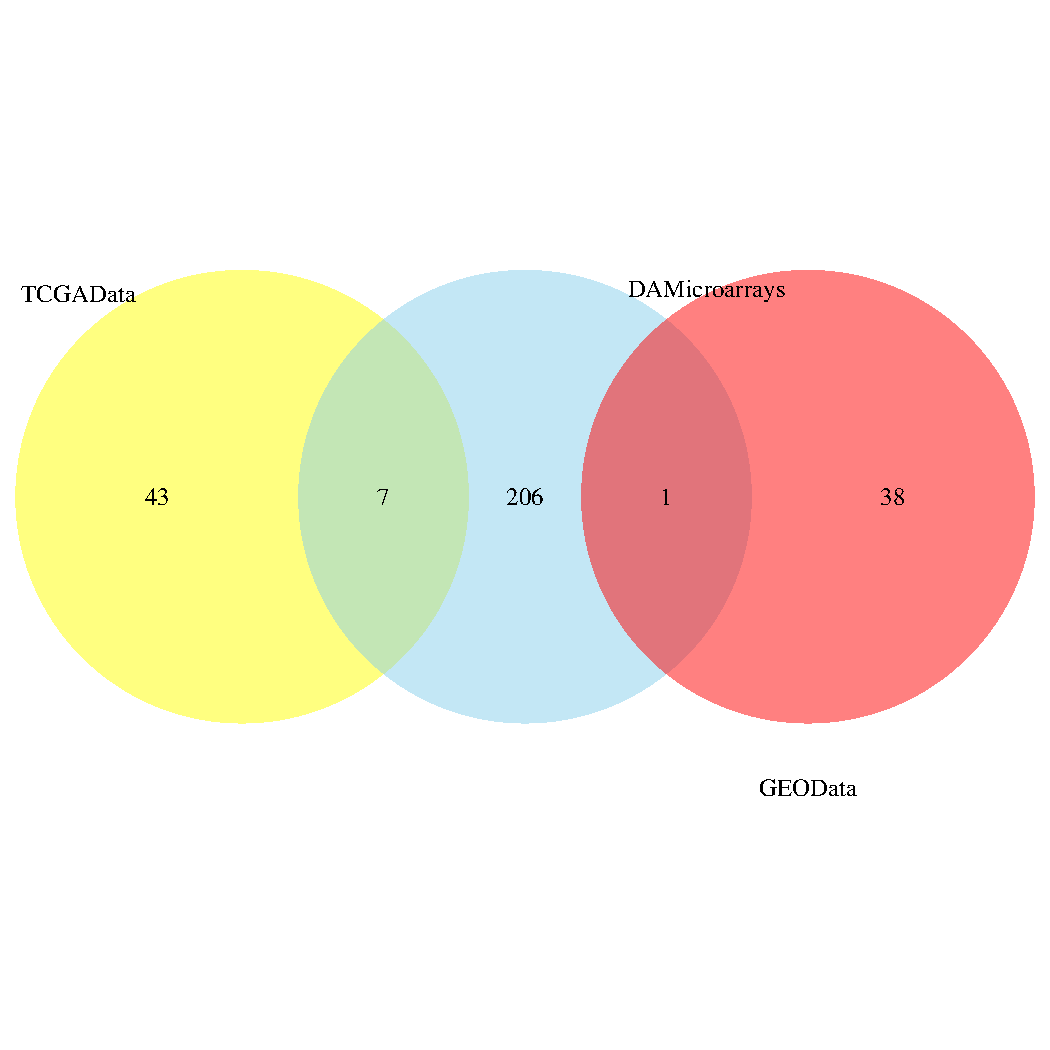
\includegraphics[width=\maxwidth]{figure/selectLGenes1-1} 
\end{knitrout}

Or it can be applied to a pre-filtered subset, such as genes showing a significantly negative correlation.


\clearpage
\begin{thebibliography}{9}

%\addcontentsline{toc}{chapter}{\numberline{}References}

\bibitem{bazzocco:2014} Sarah Bazzocco, Hafid Alazzouzi, M. Carme Ruiz de Villa, Alex Sanchez-Pla, John M. Mariadason, Diego Arango (2013) \emph{Genome-Wide Analysis of DNA Methylation in Colorectal Cancer}. Submitted.

\bibitem{Liu:2012} Yihua Liu and Peng Qiu. (2012) \emph{Integrative analysis of methylation and gene expression data in TCGA} IEEE International Workshop on Genomic Signal Processing and Statistics (GENSIPS)

\bibitem{r-project} R Development Core Team (2005). R: A language and environment for statistical computing,  reference index version 2.14.0. R Foundation for Statistical Computing, Vienna, Austria. ISBN 3-900051-07-0, \\
  \verb|http://www.R-project.org|

\bibitem{racine:2012} Jeffrey Racine. (2012) A primer on regression splines.\newline
\verb|http://cran.r-project.org/web/packages/crs/vignettes/spline_primer.pdf|

\end{thebibliography}

\end{document}
